\documentclass[preprint,review,12pt]{elsarticle}

\usepackage[utf8]{inputenc}
\usepackage[T1]{fontenc}
\usepackage{hyperref}
\usepackage{url}
\usepackage{booktabs}
\usepackage{amsfonts}
\usepackage{nicefrac}
\usepackage{microtype}
\usepackage{graphicx}
\usepackage{natbib}
\usepackage{multirow}
\usepackage{adjustbox}
\usepackage{lineno}

\linenumbers

\journal{Technological Forecasting and Social Change}

\hypersetup{
  pdftitle={When the Middle Disappears: Three Orders of AI-Driven Economic Transformation from a Multi-LLM Delphi Analysis},
  pdfkeywords={artificial intelligence, general-purpose technology, Delphi method, scenario analysis, economic transformation, large language models, foresight methodology, sociotechnical transitions},
}

\begin{document}

\begin{frontmatter}

\title{When the Middle Disappears: Three Orders of AI-Driven Economic Transformation from a Multi-LLM Delphi Analysis}

\author[anon]{[Author removed for double-blind review]}
%\cortext[cor1]{Corresponding author}
%\ead{[removed for review]}

\address[anon]{[Affiliation removed for double-blind review]}

\begin{abstract}
Existing research on AI's economic impact is bifurcated between micro-level task-substitution studies and macro-level productivity analyses, leaving a gap in understanding how effects cascade across sectors and orders of consequence. This paper introduces the Multi-LLM Delphi -- a two-round foresight method in which seven frontier language models from three geopolitical regions serve as independent, structured panelists. Applied to AI-driven economic transformation across eight GICS-aligned industry verticals, four adoption stages, and three bounding scenarios, the method yields a 114,000-word corpus analyzed through structured comparative content analysis with consensus scoring. Round 1 reveals six high-consensus convergence zones, including labor market bifurcation (7/7 models), infrastructure bottleneck repricing (6/7), and the collapse of intermediary business models (5/7). Round 2 feedback produces significant consensus dynamics: the ``apprenticeship crash'' -- the prediction that eliminating junior roles severs experiential training pipelines -- moves from 1/7 to 7/7 endorsement, though this convergence should be interpreted as an upper bound of latent consensus given LLMs' known acquiescence tendencies. Geopolitical patterns emerge along model provenance, with US-origin models emphasizing market-driven disruption, Chinese-origin models foregrounding state-steered transformation, and the single European model privileging regulatory frameworks -- patterns that warrant validation with larger model samples. Framed through General Purpose Technology theory and the Multi-Level Perspective on sociotechnical transitions, the study contributes both a cross-sector transformation map tracing AI's cascading effects from task automation through structural reorganization to systemic geopolitical consequences, and a novel methodological instrument for scalable foresight research. The findings suggest that AI's economic future is not a single trajectory but a contested, path-dependent, geopolitically differentiated process.
\end{abstract}

\begin{keyword}
artificial intelligence \sep general-purpose technology \sep Delphi method \sep scenario analysis \sep economic transformation \sep large language models \sep foresight methodology \sep sociotechnical transitions
\end{keyword}

\end{frontmatter}


\section{Introduction}
\label{sec:introduction}

In 2024, over 78 percent of organizations worldwide reported using artificial intelligence in at least one business function, up from 55 percent just one year earlier \citep{mckinsey2025ai}. Global investment in AI infrastructure was projected to surpass three hundred billion dollars in combined hyperscaler capital expenditure \citep{morganstanley2024capex}, and data center electricity demand was projected to potentially more than double by 2026 under high-growth scenarios \citep{iea2024electricity}. These figures signal that AI is no longer an emerging technology but an active force reshaping the productive apparatus of the global economy. Yet the scholarly understanding of \textit{what, precisely, this reshaping will look like} across sectors, stages, and systemic levels remains fragmented.

The fragmentation reflects a structural limitation in the literature. Labor economists model task-level substitution \citep{acemoglu2018artificial, acemoglu2019automation, acemoglu2022aijobs, eloundou2023gpts, autor2024applying, frank2019toward} and provide rigorous estimates of exposure but typically bracket the structural and systemic consequences that unfold once substitution reaches scale. Management scholars examine firm-level adoption dynamics \citep{raisch2021automation, kanbach2023genai, dwivedi2023chatgpt} but rarely extend analysis to cross-sector convergence effects or geopolitical restructuring. Foresight researchers employ Delphi studies and scenario analysis to map transformation pathways \citep{culot2020manufacturing, fritschy2019autonomous}, but their human expert panels are limited in scale, subject to desirability bias \citep{ecken2011desirability}, and constrained by the availability and self-selection of panelists \citep{foerster2014delphipanel, sokolov2025delphias}.

What is missing is an analytical framework that (a) traces effects across multiple orders of consequence -- from immediate task automation (first order) through structural reorganization of industries, value chains, and labor markets (second order) to systemic geopolitical and civilizational transformation (third order) -- (b) does so across a comprehensive set of industry verticals rather than a single sector, and (c) uses a scalable methodology that can capture diverse expert perspectives without the practical constraints of assembling large human panels.

This paper addresses the gap with two interlinked contributions. The \textbf{primary contribution is substantive}: a comprehensive, cross-sector map of AI-driven economic transformation that traces cascading effects across three orders of consequence. Seven frontier language models -- representing three geopolitical regions (US, China, EU) and seven corporate ecosystems -- independently analyzed AI transformation across eight GICS-aligned industry verticals, four sequential adoption stages, three bounding scenarios, and three orders of effects. The resulting 114,000-word corpus, consolidated through structured comparative content analysis with consensus scoring, identifies six high-consensus convergence zones where the transformation literature's predictions are cross-examined through structured multi-model comparison, alongside contested futures and blind spots that reveal where genuine uncertainty persists. The most striking substantive finding is the ``apprenticeship crash'' -- the prediction that AI's elimination of junior knowledge-work roles will sever the experiential pipeline through which senior professionals are produced, creating a judgment famine within a decade. Initially identified by only one model, this prediction achieved unanimous endorsement across all seven models after controlled feedback, suggesting it represents a systematically underappreciated structural risk.

The \textbf{secondary contribution is methodological}: the Multi-LLM Delphi, a novel foresight instrument in which multiple frontier AI language models serve as independent, structured panelists in a two-round design with controlled feedback \citep{linstone1975delphi, gordon2006rtdelphi}. The epistemological foundation treats frontier LLMs as structured knowledge synthesizers -- their outputs represent recombinative syntheses of academic, industry, and policy knowledge, subject to known biases (training data composition, RLHF alignment, and regional training data skews) that themselves become analytically informative when compared across model families (see Section~\ref{sec:epistemological_status} for the epistemological framework). The method's comparative advantage lies not in replacing human expertise but in providing rapid, scalable, and structurally diverse reconnaissance of complex transformation landscapes.

Three research questions guide the analysis:

\textbf{RQ1:} What first-, second-, and third-order effects of AI-driven transformation do frontier LLMs project across eight industry verticals under MILD, BASE, and MAX scenarios?

\textbf{RQ2:} Which second- and third-order effects converge across verticals into systemic tipping points, and what wildcards emerge?

\textbf{RQ3:} What methodological properties does the Multi-LLM Delphi exhibit -- where do model families converge, diverge, and show geopolitically differentiated perspectives?

The paper contributes to the literature on technological forecasting and social change in three ways. First, it provides a methodological innovation that extends the Delphi tradition into the era of frontier AI, offering a scalable complement to human expert panels. Second, it generates directional foresight content -- a comprehensive transformation map that policymakers, industry strategists, and researchers can use to anticipate cascading effects. Third, it demonstrates radical transparency in AI-assisted research by fully documenting the data collection process and the role of AI tools in the research workflow.

The paper is structured as follows. Section 2 reviews the theoretical foundations: General Purpose Technology theory, the Multi-Level Perspective on sociotechnical transitions, and the Delphi methodology literature. Section 3 describes the Multi-LLM Delphi method in detail, including the two-round protocol. Section 4 presents results: Sections 4.1 through 4.4 report Round 1 findings organized by consensus level (high-consensus convergence zones, contested futures, blind spots, and geopolitical divergence), while Section 4.5 reports Round 2 consensus dynamics under controlled feedback. Section 5 discusses theoretical, methodological, and practical implications. Section 6 addresses limitations and future research directions, and Section 7 concludes.



\section{Theoretical Background}
\label{sec:theoretical_background}


\subsection{Artificial Intelligence as General Purpose Technology}
\label{sec:ai_as_gpt}

The concept of a general-purpose technology (GPT) was formalized by \citet{bresnahan1995gpt} to describe technologies exhibiting three defining characteristics: pervasive applicability across economic sectors, persistent technological improvement over time, and the capacity to generate complementary innovations in adopting sectors. Canonical examples include the steam engine, electricity, and the internal combustion engine -- technologies whose transformative impact unfolded not through direct application alone but through the cascading structural changes they enabled across the entire economy.

\citet{brynjolfsson2017productivity} applied the GPT framework to artificial intelligence and introduced the concept of the AI productivity paradox: the observation that AI is simultaneously "everywhere in discourse but nowhere in the statistics," paralleling the Solow paradox observed during the early diffusion of information technology. The resolution, they argued, lies in the J-curve of GPT adoption -- an initial period of investment, reorganization, and intangible capital accumulation that depresses measured productivity, followed by an inflection point at which productivity gains accelerate. This J-curve logic provides the theoretical foundation for the four-stage adoption model constructed for this study: augmentation (Stage 1), where AI operates as a copilot within existing structures; reorganization (Stage 2), where processes and organizational forms adapt to AI capabilities; reinvention (Stage 3), where AI-native business models displace legacy structures; and systemic transformation (Stage 4), where economy-wide restructuring alters labor markets, geopolitics, and power structures.

The GPT framework further predicts that the most economically significant effects of a general-purpose technology are not its direct applications but the complementary innovations and structural changes it enables \citep{bresnahan1995gpt, korzinov2018gpt, coccia2018longwaves}. Applied to AI, this means that the first-order effects -- task-level productivity gains from AI copilots -- are economically important but represent only the visible surface of a deeper transformation. The second-order effects -- reorganization of value chains, business models, and labor market structures -- and the third-order effects -- systemic shifts in geopolitical power, regulatory regimes, and social contracts -- are where the GPT framework predicts the largest and most consequential changes will occur. This prediction motivates the three-order analytical framework employed in this study.

Recent empirical work has begun to validate the GPT characterization of AI. \citet{eloundou2023gpts} estimated pervasive applicability, finding that approximately 80 percent of the US workforce could have at least 10 percent of their tasks exposed to LLMs. \citet{brynjolfsson2023generative} documented persistent improvement by showing that AI tools substantially increase the productivity of less-experienced customer service workers. The capacity to generate complementary innovations is visible in the emergence of new roles (prompt engineers, AI orchestrators), new business models (AI-as-a-service, outcome-based pricing), and new organizational forms \citep{kanbach2023genai, brown2024theory}.


\subsection{The Multi-Level Perspective on Sociotechnical Transitions}
\label{sec:mlp}

While GPT theory explains \textit{why} AI transformation cascades across sectors and generates higher-order effects, it provides limited analytical purchase on the \textit{mechanisms} through which these transformations unfold -- the role of incumbent resistance, regulatory intervention, cultural adaptation, and path dependency. For this, we draw on the Multi-Level Perspective (MLP) on sociotechnical transitions \citep{geels2005coevolutionary, geels2011multilevel, geels2020microfoundations}.

The MLP distinguishes three analytical levels: the niche, where radical innovations emerge and are sheltered from mainstream market selection; the sociotechnical regime, the dominant configuration of technologies, institutions, practices, and rules that stabilize existing systems; and the landscape, the exogenous macro-level context (macroeconomic trends, geopolitical shifts, cultural values) that creates pressure on regimes. Transitions occur when niche innovations align with landscape pressures to destabilize incumbent regimes, creating windows of opportunity for structural change \citep{geels2011multilevel, roberts2019accelerated}.

The MLP maps onto the analytical framework of this study as follows. Stage 1 (Augmentation) corresponds to niche-level innovation: AI tools operate within existing organizational and institutional structures, producing efficiency gains without challenging the incumbent regime. Stage 2 (Reorganization) represents the beginning of regime destabilization: AI capabilities become sufficiently mature to trigger organizational restructuring, new business models, and shifts in competitive dynamics. Stage 3 (Reinvention) corresponds to full regime disruption: AI-native organizations and business models displace legacy structures, and the sociotechnical configuration of entire industries is reconfigured. Stage 4 (Systemic Transformation) represents landscape-level change: the cumulative effects of AI adoption across multiple sectors alter geopolitical power structures, labor market institutions, and the social contract itself \citep{geels2020microfoundations, geels2020scenarios, walrave2018mlp}.

Critically, the MLP predicts that transitions are not smooth or deterministic. They are contested, path-dependent, and shaped by the agency of incumbents, regulators, and social movements \citep{geels2020microfoundations, kern2012mlppolicy}. Different societies may traverse the same technological transition through different pathways, at different speeds, and with different outcomes -- a prediction that provides the theoretical rationale for examining geopolitical divergence in model outputs.


\subsection{The Delphi Method and Its Extensions}
\label{sec:delphi_method}

The Delphi method, originally developed at the RAND Corporation in the 1950s, elicits structured expert judgments through iterative anonymous questionnaires with controlled feedback \citep{gordon2006rtdelphi}. The method has been extensively applied in technological forecasting and scenario analysis, with particular relevance for contexts where empirical data is scarce and expert judgment must substitute for direct observation \citep{culot2020manufacturing, fritschy2019autonomous, stahl2023chatgpt}.

Central to Delphi quality is the measurement of consensus. \citet{vondergracht2012delphi} reviewed consensus measurement practices in 80 Delphi studies published in \textit{Technological Forecasting and Social Change} and identified a range of approaches, including interquartile range, coefficient of variation, and percentage agreement thresholds. The study recommended that researchers define consensus criteria ex ante and report both consensus and dissensus findings, as divergence patterns can be as analytically informative as convergence.

The Delphi method faces well-documented limitations. Desirability bias causes panelists to overestimate the likelihood of outcomes they consider beneficial \citep{ecken2011desirability}. Panel composition effects arise from the inherent difficulty of assembling genuinely diverse expert groups; panels tend to over-represent readily available experts and under-represent perspectives from underrepresented regions or disciplines \citep{foerster2014delphipanel, sokolov2025delphias}. Expert availability constraints limit panel size and impose practical ceilings on the breadth of expertise that can be mobilized.

Recent work has begun exploring the intersection of large language models and research methodology. \citet{grybauskas2024llm} used LLMs to analyze employer perspectives on Industry 5.0 in a study published in \textit{Technological Forecasting and Social Change}, demonstrating the potential of LLMs as analytical instruments. \citet{guo2026llmsynthesis} employed LLMs for automatic synthesis of econometric results. \citet{liu2026llmsupplychain} explored LLM integration in supply chain research. These studies suggest a growing acceptance of LLMs as research tools, though none has employed multiple LLMs as \textit{panelists} in a formal multi-round Delphi design with consensus scoring.

More directly relevant to the present study, \citet{calleo2025rtaidelphi} proposed a ``Real-Time AI Delphi'' that integrates a single AI model into the continuous Delphi framework for decision-making contexts. \citet{mostashari2025aivisions} used multiple AI platforms in a Delphi-like approach to generate future scenarios for AI development, though without formal consensus scoring or controlled multi-round feedback. On the substantive side, \citet{acemoglu2024simplemacro} modeled the aggregate macroeconomic effects of AI using a task-based framework, concluding that first-order productivity gains alone are unlikely to generate transformative GDP growth --- a finding that underscores the importance of examining higher-order structural effects, as this study does. \citet{bail2024genaisocialscience} provided a comprehensive framework for integrating generative AI into social science research, while \citet{crockett2024llmparticipants} raised critical concerns about substituting LLMs for human research participants, identifying epistemological limitations that the present study addresses through the ``structured knowledge synthesis'' framework developed in Section~\ref{sec:epistemological_status}.

What remains absent from this literature is an approach that simultaneously (a) uses multiple LLMs from different providers and geopolitical origins as structured, independent panelists in a multi-round protocol, (b) maps AI transformation across a comprehensive set of industry verticals through three orders of cascading effects, and (c) provides formal consensus measurement with geopolitical divergence analysis. Table~\ref{tab:positioning} summarizes the positioning of the Multi-LLM Delphi relative to the closest existing approaches.

\begin{table}[htbp]
\centering
\caption{Positioning of the Multi-LLM Delphi Relative to Existing Approaches}
\label{tab:positioning}
\adjustbox{max width=\textwidth}{%
\begin{tabular}{p{3.2cm}p{2.5cm}p{2.5cm}p{2.5cm}p{2.5cm}p{3cm}}
\toprule
\textbf{Feature} & \textbf{Classical Delphi} & \textbf{RT-Delphi} \scriptsize{\citep{gordon2006rtdelphi}} & \textbf{AI Delphi} \scriptsize{\citep{calleo2025rtaidelphi}} & \textbf{Multi-AI Scenarios} \scriptsize{\citep{mostashari2025aivisions}} & \textbf{Multi-LLM Delphi} \scriptsize{(This paper)} \\
\midrule
Panelists & Human experts (10--30) & Human experts (continuous) & Single AI + humans & Multiple AI platforms & 7 frontier LLMs \\
Rounds & 3--4 & Continuous & Real-time & Not specified & 2 (controlled) \\
Feedback & Anonymized statistics & Continuous, visible & AI-integrated & Informal & Anonymized consensus summary \\
Independence & Anonymous & Partially visible & Hybrid & Unclear & Fully independent \\
Geopolitical diversity & Recruitment-dependent & Recruitment-dependent & None & Limited & Built-in (US/CN/EU) \\
Effect depth & Domain-specific & Domain-specific & Single-order & Scenario-level & 3 orders (cascading) \\
Sector scope & Typically 1--2 & 1--2 & Domain-specific & AI sector only & 8 GICS verticals \\
Consensus scoring & IQR, \% agreement & Continuous stats & Built-in & None reported & HC/MC/CF/BS system \\
Bias analysis & Limited & Limited & Limited & None & Extensive (acquiescence) \\
\bottomrule
\end{tabular}%
}
\end{table}

A brief note on the ``Delphi'' label is warranted. Classical Delphi is defined by iterative rounds with controlled feedback \citep{linstone1975delphi}. This study implements a two-round design with controlled feedback: Round 1 collects independent structured judgments, and Round 2 provides anonymized consensus summaries and solicits revisions, adoptions, and contestations. This protocol satisfies the core procedural requirement of classical Delphi -- structured elicitation followed by controlled feedback and revision opportunity -- while substituting computational panelists for human ones. The Delphi tradition has also moved beyond strict multi-round iteration as a constitutive requirement. \citet{gordon2006rtdelphi} introduced Real-Time Delphi (RT-Delphi), which eliminates discrete rounds entirely in favor of continuous asynchronous updating, demonstrating that the core of the method lies in structured expert elicitation with controlled diversity rather than in any specific number of iterations. What defines the Delphi family is an epistemological commitment: the systematic aggregation of independent, structured judgments from diverse sources to map areas of consensus and dissensus, with feedback mechanisms that allow panelists to revise their positions in light of peer perspectives. The Multi-LLM Delphi preserves this commitment -- seven independent models, queried with identical instruments, producing outputs that are systematically compared for convergence and divergence, with a feedback round that enables revision. We use ``Delphi'' as a conceptual anchor to locate the method within the foresight tradition, while acknowledging important epistemological differences between LLM and human panelists that are discussed in Section 5.

The Multi-LLM Delphi method introduced in this paper is best understood as a \textit{Delphi-inspired} instrument that adapts the tradition's core procedural logic -- structured elicitation, controlled feedback, consensus measurement -- while substituting a fundamentally different type of panelist. It does not claim to extend the Delphi method in the sense of adding a new variant to the existing family; rather, it transplants the Delphi's procedural architecture into a new epistemic context (LLM-generated outputs) where important properties of classical Delphi -- embodied expertise, professional stakes, genuine belief revision -- are absent, and different properties -- scalability, structural diversity through model provenance, reproducibility -- are present. The method uses frontier AI models as structured knowledge synthesizers rather than surrogate experts. The epistemological justification is that frontier LLMs are trained on vast corpora of academic, industry, and policy literature; their outputs represent probabilistic syntheses of this knowledge, shaped by known biases (training data composition, RLHF alignment, and regional data skews). By querying multiple models from different providers, regions, and corporate ecosystems, the method generates structured diversity analogous to -- though fundamentally different from -- the diversity sought in traditional expert panels. The key analytical move is to treat model agreement as a measure of epistemic convergence across training corpora, and model disagreement as a signal of either genuine uncertainty, knowledge gaps, or systematic bias traceable to model provenance.


\subsection{Epistemological Status of LLM-Generated Predictions}
\label{sec:epistemological_status}

A central question for the Multi-LLM Delphi --- and one that distinguishes it from traditional Delphi studies --- concerns the epistemic status of the outputs it produces. Human experts bring embodied experience, professional stakes, and domain-specific judgment to Delphi panels. LLMs bring something categorically different: a compressed, probabilistic representation of their training corpora, shaped by architectural choices and alignment procedures. Understanding what LLM consensus \textit{means} requires articulating what LLMs \textit{are} in epistemological terms.

We propose a framework that positions LLM outputs along a spectrum between two poles, neither of which fully captures the phenomenon. At one pole is the \textbf{``stochastic parrot'' interpretation} \citep{bender2021parrots}: LLMs merely reproduce statistical regularities in text without understanding, and their consensus reflects nothing more than the co-occurrence of claims in widely available documents. Under this interpretation, the Multi-LLM Delphi is an elaborate literature survey --- useful for mapping the distribution of existing claims but incapable of generating genuine analytical insight. At the other pole is the \textbf{``synthetic expert'' interpretation}: LLMs have internalized sufficient knowledge to perform genuine reasoning about complex domains, and their consensus reflects analytical convergence analogous to human expert agreement. Under this interpretation, the Multi-LLM Delphi is a direct substitute for human expert panels.

Neither pole is defensible in isolation. The stochastic parrot position cannot account for the documented capacity of LLMs to perform novel causal reasoning, solve unseen problems, and generate predictions that do not appear verbatim in their training data \citep{wei2022emergent, bubeck2023sparks}. The apprenticeship crash prediction in this study illustrates this: only one model generated it spontaneously in Round~1, but all seven models could reconstruct its causal logic independently once prompted --- suggesting that the underlying reasoning capability was present but not activated, rather than absent. Conversely, the synthetic expert position overstates LLM capabilities by ignoring that models lack embodied experience, cannot update their knowledge in real time, and are subject to well-documented biases including sycophancy, hallucination, and training data skew \citep{perez2023sycophancy, sharma2024sycophancy}.

We adopt an intermediate position that we term the \textbf{``structured knowledge synthesis'' interpretation.} Under this view, each frontier LLM constitutes a compressed, partial, and biased --- but analytically productive --- encoding of its training corpus, filtered through its architectural and alignment characteristics. The outputs are neither raw reproduction nor genuine expertise, but a form of \textit{structured recombination}: the model assembles existing knowledge elements into novel configurations guided by the prompt structure, producing outputs that are constrained by but not reducible to the training data. This interpretation has three implications for the Multi-LLM Delphi:

First, \textbf{LLM consensus signals epistemic density, not truth.} When multiple independently trained models converge on a prediction, this indicates that the prediction is well-supported across diverse knowledge corpora --- a form of triangulation across information sources. It does not guarantee that the prediction is correct, but it does indicate that the claim is robust to variation in training data, architecture, and alignment. This is analogous to the classical Delphi interpretation of consensus as ``informed convergence'' rather than proof \citep{linstone1975delphi}.

Second, \textbf{LLM disagreement signals either genuine uncertainty or systematic bias.} When models diverge, the divergence may reflect genuine epistemic uncertainty about the future (as with the pace of healthcare transformation) or systematic differences in training data composition (as with the geopolitical divergence pattern). The Multi-LLM Delphi's analytical power lies precisely in this diagnostic capacity: by comparing outputs from models with known provenance differences, it can distinguish informational uncertainty from institutional bias.

Third, \textbf{the Multi-LLM Delphi is best understood as a complementary instrument, not a replacement for human expertise.} Its comparative advantage lies in breadth (systematic coverage of a large analytical space), speed (hours rather than months), reproducibility (identical prompts across panelists), and structural diversity (geopolitical variation achieved through model selection). Its limitation lies in depth: LLMs cannot contribute the tacit knowledge, professional stakes, and identity-based commitments that anchor human expert judgment. The optimal deployment is as a first-round scanning instrument that maps the landscape and identifies areas where human expert judgment is most needed --- a ``computational reconnaissance'' that complements rather than substitutes for traditional foresight methods.


\subsection{Scenario Analysis and Orders of Effects}
\label{sec:scenario_analysis}

Scenario analysis is a structured approach to exploring multiple plausible futures \citep{vanderheijden1996scenarios, postma2005scenario}. Unlike forecasting, which aims to predict a single most likely outcome, scenario analysis develops bounding cases that span the space of plausible outcomes, enabling decision-makers to prepare for multiple contingencies \citep{banuls2011scenario}. The combination of Delphi methodology with scenario analysis has a strong tradition in \textit{Technological Forecasting and Social Change}, where studies have used expert panels to develop and evaluate scenarios for Industry 4.0 \citep{culot2020manufacturing}, autonomous transportation \citep{fritschy2019autonomous}, and sustainability transitions \citep{geels2020scenarios}.

The three-order framework used in this study draws on historical analogy. First-order effects are immediate and directly visible (the automobile created demand for gasoline stations). Second-order effects are structural consequences that emerge when first-order adoption reaches scale (the automobile enabled suburbs, highway infrastructure, and the restructuring of retail around automobile accessibility). Third-order effects are systemic and civilizational, emerging from the compound interaction of first- and second-order changes in ways that were near-impossible to predict from the original innovation (the automobile transformed the geopolitics of the Middle East through oil demand). Applied to AI, the framework systematically traces effects from task automation through organizational restructuring to geopolitical and social transformation. Figure~\ref{fig:cascade} illustrates this cascade logic.

\begin{figure}[htbp]
\centering

\includegraphics[width=\textwidth,height=0.88\textheight,keepaspectratio]{figures/fig5_cascade.png}
\caption{Three-Order Effect Cascade with Historical Automobile Parallel. First-order effects (task automation) cascade into second-order effects (structural reorganization of value chains, labor markets, and business models) and third-order effects (systemic shifts in geopolitical power, regulatory regimes, and social contracts). The right track shows the historical automobile analogy. Model consensus decreases from first-order (7/7) to third-order (3--5/7) effects, reflecting increasing uncertainty about long-term systemic outcomes.}
\label{fig:cascade}
\end{figure}


\section{Method}
\label{sec:method}


\subsection{Research Design}
\label{sec:research_design}

This study employs a two-round Multi-LLM Delphi design. In Round 1, the author queried seven frontier language models in parallel with an identical structured prompt, then consolidated their outputs through structured comparative content analysis with consensus scoring. In Round 2, each model received the anonymized consensus summary and a structured revision prompt. This design implements the core Delphi principle of controlled feedback \citep{linstone1975delphi} within a multi-LLM architecture, enabling assessment of consensus dynamics, blind-spot adoption, and the stability of divergence patterns under feedback pressure. Figure~\ref{fig:methodology} provides an overview of the complete research design.

\begin{figure}[htbp]
\centering
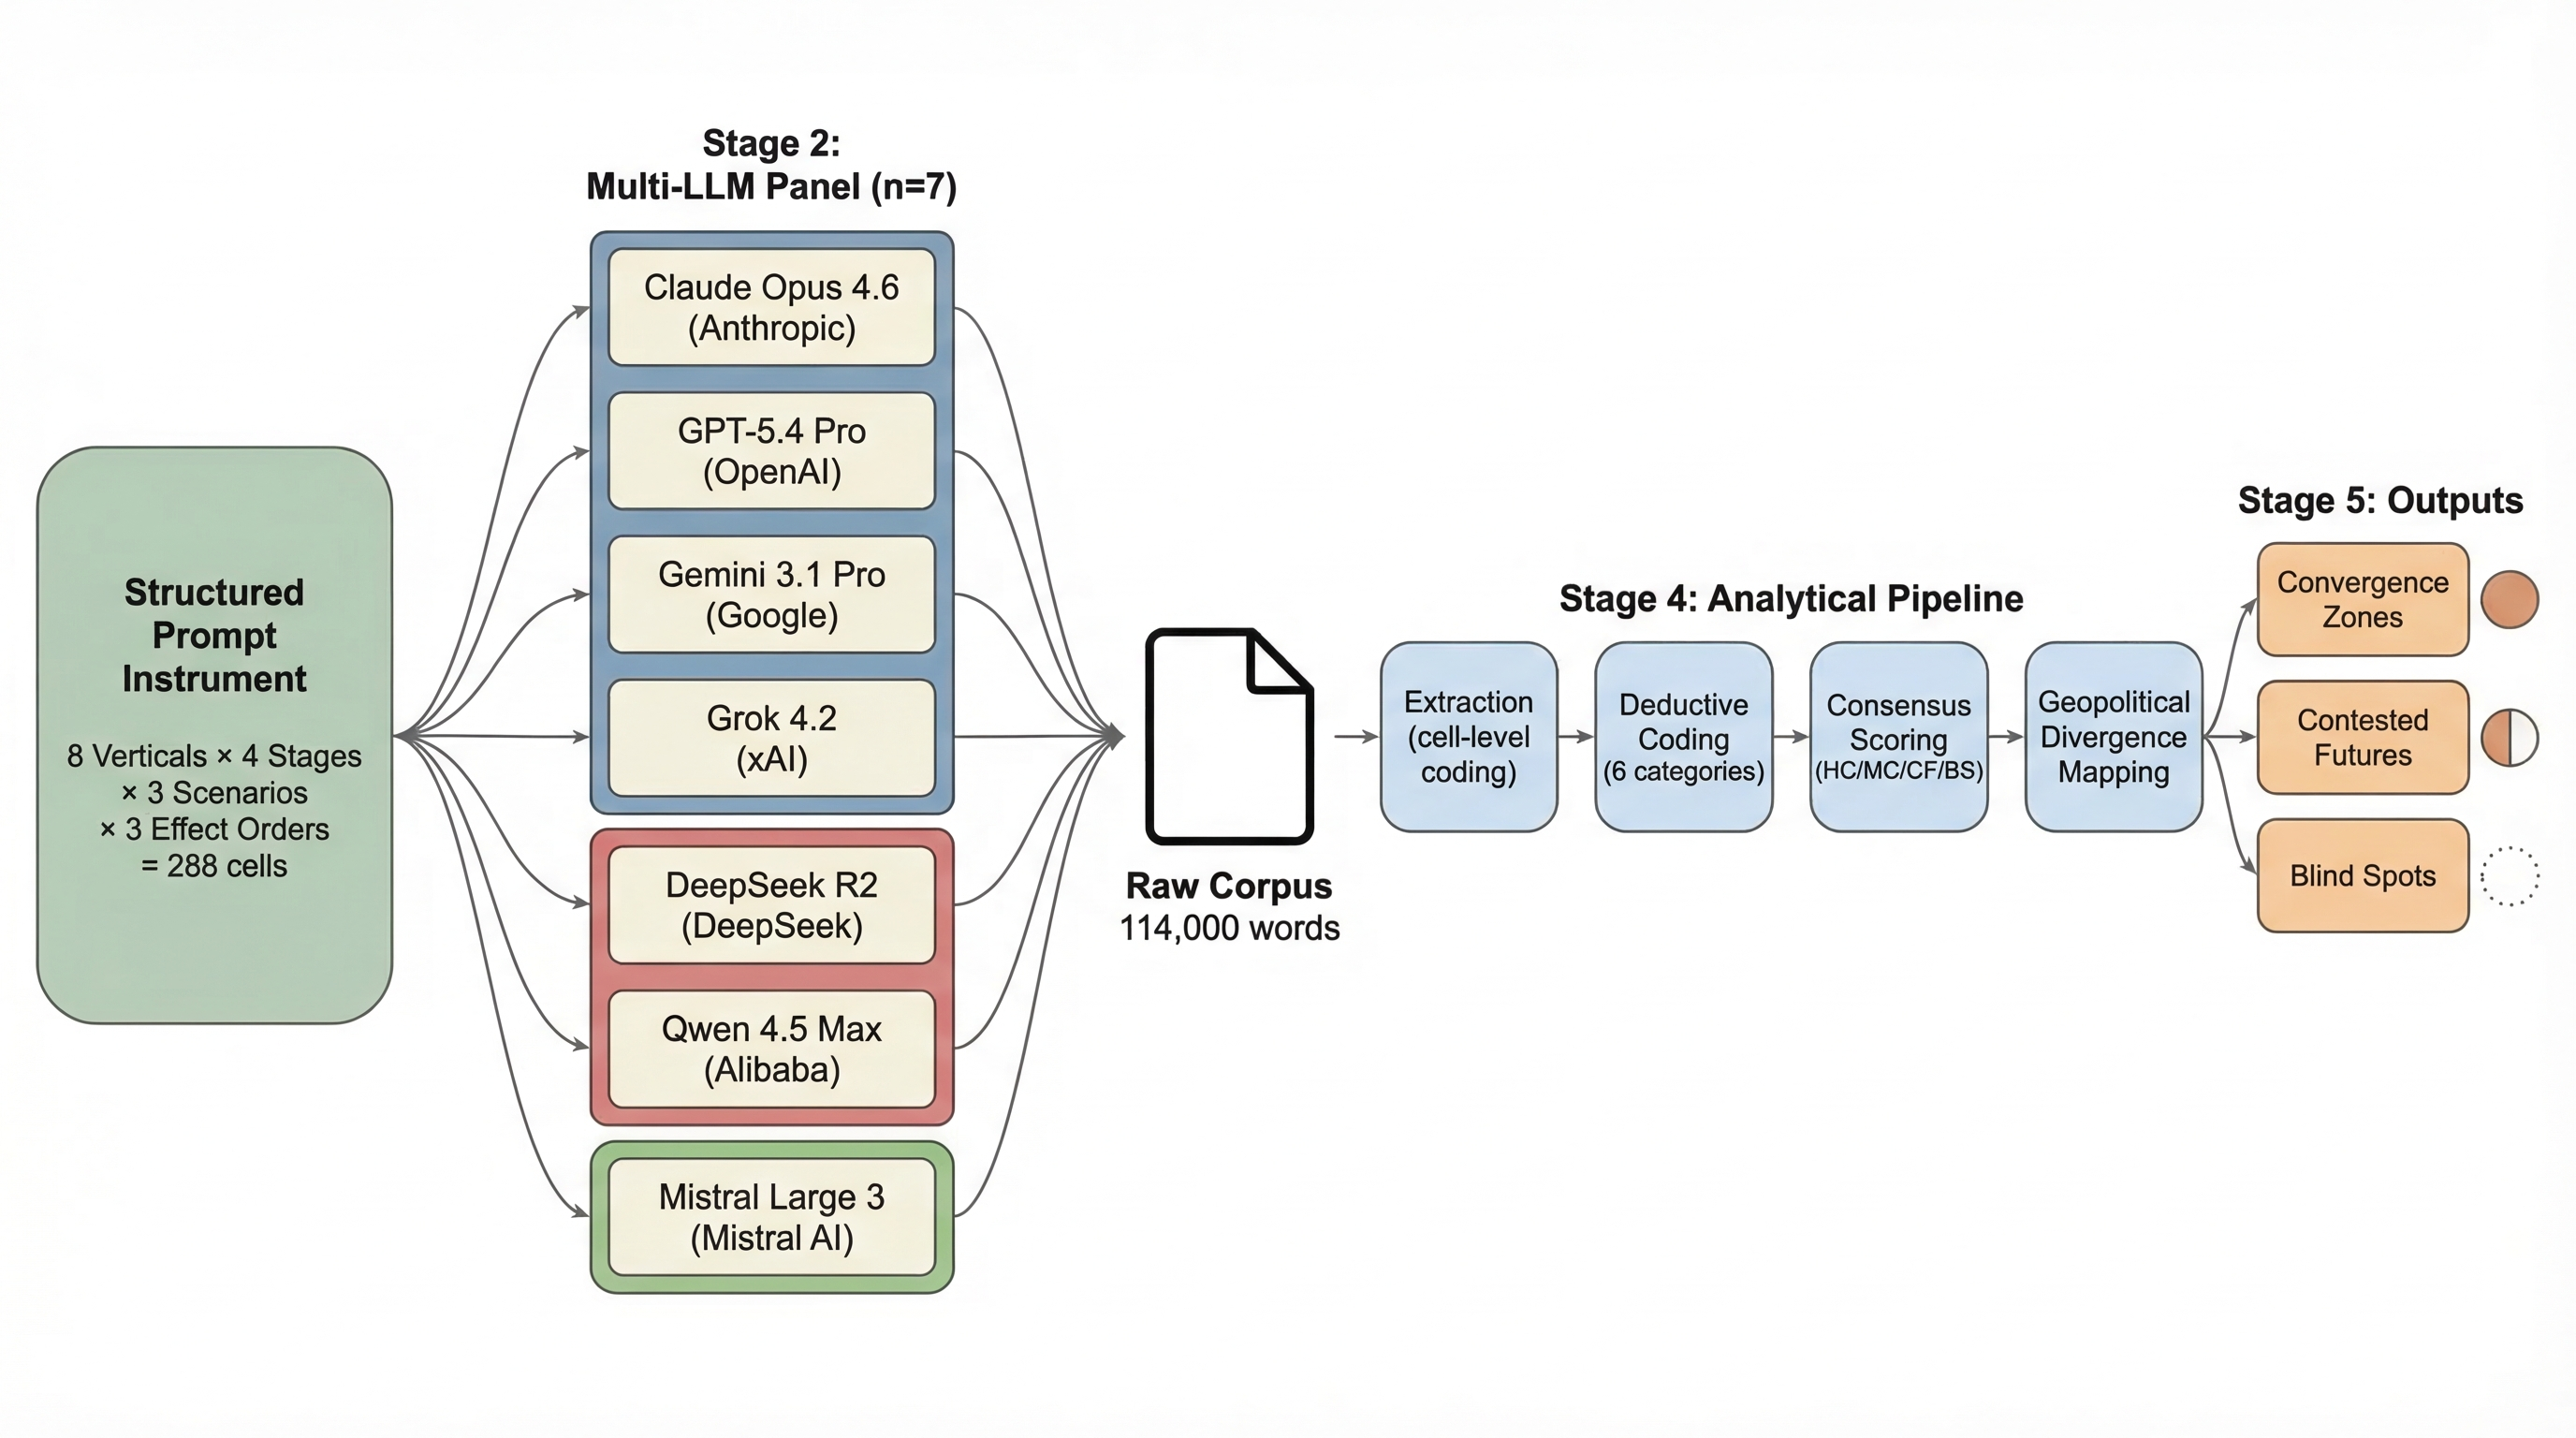
\includegraphics[width=\textwidth,height=0.85\textheight,keepaspectratio]{figures/fig1_methodology.png}
\caption{Multi-LLM Delphi Research Design. Seven frontier language models from three geopolitical regions (US: blue, CN: red, EU: green) are queried in parallel with an identical structured prompt instrument specifying 288 analytical cells. The 114,000-word corpus is processed through a four-step analytical pipeline, yielding convergence zones, contested futures, and blind spots.}
\label{fig:methodology}
\end{figure}


\subsection{Model Selection and Panel Composition}
\label{sec:model_selection}

The author selected seven frontier models to maximize diversity across three dimensions: corporate ecosystem (no two models from the same parent organization), geographic origin (representing US, Chinese, and European AI development trajectories), and architectural approach (spanning different training philosophies and alignment strategies). Table~\ref{tab:panel_composition} summarizes the panel composition.

\begin{table}[htbp]
\centering
\caption{Multi-LLM Delphi Panel Composition}
\label{tab:panel_composition}
\adjustbox{max width=\textwidth}{%
\begin{tabular}{llllll}
\toprule
\textbf{Model} & \textbf{Provider} & \textbf{HQ Region} & \textbf{Architecture} & \textbf{Release} & \textbf{Role in Panel} \\
\midrule
Claude Opus 4.6 & Anthropic & US & Constitutional AI, 1M context & Feb 2026 & US perspective, safety-aligned \\
GPT-5.4 & OpenAI & US & Advanced reasoning, 1M context & Mar 2026 & US perspective, market leader \\
Gemini 3.1 Pro & Google DeepMind & US & Deep Think mode, agentic workflows & Feb 2026 & US perspective, data-rich \\
Grok 4.2 & xAI & US & Parallel test-time compute, X integration & 2026 & US perspective, contrarian \\
DeepSeek R2 & DeepSeek & China & MoE, reasoning-optimized & Feb 2026 & Chinese perspective, technical \\
Qwen 4.5 Max & Alibaba Cloud & China & Multilingual, vision-language, agentic & Jan 2026 & Chinese perspective, industrial \\
Mistral Large 3 & Mistral AI & EU (France) & 675B parameters, open-weight heritage & Late 2025 & European perspective, regulatory-aware \\
\bottomrule
\end{tabular}}%
\end{table}

The geographic distribution (4 US, 2 Chinese, 1 EU) reflects the current landscape of frontier AI development rather than a balanced design. This asymmetry is acknowledged as a limitation and is analytically productive: it enables assessment of within-family convergence among US models and between-family divergence across geopolitical blocs.


\subsection{Prompt Instrument}
\label{sec:prompt_instrument}

The author developed a standardized structured prompt as the research instrument (the full prompt is available in the supplementary materials). The prompt specified:

\begin{enumerate}
  \item \textbf{Role framing:} "You are a senior economic analyst and futures researcher."
  \item \textbf{Conceptual framework:} Three orders of effects (with automobile analogy for calibration), three bounding scenarios (MILD, BASE, MAX), four sequential adoption stages (Augmentation, Reorganization, Reinvention, Systemic Transformation), and eight GICS-aligned industry verticals.
  \item \textbf{Output structure:} For each of the 8 verticals x 4 stages, a structured table with cells for each scenario x effect order combination, plus roles eliminated, roles created, and critical skills.
  \item \textbf{Cross-cutting analysis:} Cross-vertical convergence points, wildcard scenarios, and synthesis on the human dimension.
  \item \textbf{Style directives:} Declarative language, named companies and technologies, causal chain reasoning, no hedging.

\end{enumerate}
The author designed the prompt to be maximally structured while leaving substantive content generation entirely to the models. No examples, priming data, or desired conclusions were included. The "chain of events" reasoning directive forced models to articulate causal mechanisms rather than produce generic predictions.


\subsection{Data Collection}
\label{sec:data_collection}

The author conducted the data collection on March 14--15, 2026. Each model received the identical structured prompt through its native chat interface (claude.ai, chatgpt.com, gemini.google.com, grok.x.ai, chat.deepseek.com, qwen.alibaba.com, and chat.mistral.ai) in a fresh conversation. This approach ensured that each model operated with its default parameters, full context window, and standard safety settings, avoiding potential API-specific truncation, temperature manipulation, or parameter artifacts that could introduce systematic bias. The trade-off is reduced reproducibility, as native interface responses may vary across sessions. Importantly, the substantial output length variation documented in Section~\ref{sec:methodological_properties} (14:1 ratio between longest and shortest response) may partly reflect differences in default parameters (temperature, maximum output tokens, context window utilization) across interfaces rather than genuine differences in analytical depth. This confound cannot be resolved without API-based replication with standardized parameters, which the author identifies as a priority for future research.

The seven responses yielded a total corpus of approximately 114,000 words, with substantial variation in output length: Claude Opus 4.6 (30,613 words), GPT-5.4 (23,346), DeepSeek R2 (22,614), Gemini 3.1 Pro (16,330), Qwen 4.5 Max (11,024), Mistral Large 3 (8,261), and Grok 4.2 (2,169). The response length variation itself constitutes a finding about model behavior under identical prompts -- discussed in Section 4.4.


\subsection{Analytical Procedure}
\label{sec:analytical_procedure}

The author conducted a structured comparative content analysis with consensus scoring in four steps:

\textbf{Step 1: Extraction.} The author converted each model's output from its native format (.docx) to structured text using pandoc. For each analytical cell (Vertical x Stage x Effect Order x Scenario), the core prediction, named actors, causal mechanism, and intensity were extracted.

\textbf{Step 2: Deductive Coding.} The author coded predictions along four dimensions: (a) the core claim (what is predicted to happen), (b) the specificity level (generic statement vs. named actors and quantified mechanisms), (c) the causal chain quality (presence/absence of explicit causal reasoning), and (d) the thematic category (labor displacement, market concentration, regulatory response, infrastructure bottleneck, geopolitical shift, identity transformation). The complete codebook with category definitions, inclusion/exclusion criteria, decision rules for borderline cases, and worked coding examples is available in the supplementary repository (see Data Availability Statement).

\textbf{Step 3: Consensus Scoring.} Adapted from Delphi consensus measurement \citep{vondergracht2012delphi}, convergence was assessed at the thematic level across models:

\begin{itemize}
  \item \textbf{High Consensus (HC):} Five or more of seven models converge on the same thematic claim within an analytical cell or cross-cutting theme.
  \item \textbf{Moderate Consensus (MC):} Three to four models converge.
  \item \textbf{Contested Future (CF):} Models split approximately evenly, with identifiable clusters taking opposing positions.
  \item \textbf{Blind Spot (BS):} A prediction appears in only one or two models, representing either genuine novelty or idiosyncratic bias.

\end{itemize}
\textbf{Step 4: Geopolitical Divergence Mapping.} Systematic comparison across model families (US: Claude, GPT-5.4, Gemini, Grok; CN: DeepSeek, Qwen; EU: Mistral) to identify patterns of divergence traceable to geographic origin rather than random variation.


\subsection{Round 2 Protocol: Controlled Feedback and Iterative Revision}
\label{sec:round2_protocol}

Following the Round 1 analysis, the author administered a structured Round 2 prompt to all seven models. The protocol proceeded in three stages.

\textbf{Stage 1: Consensus Summary Preparation.} The Round 1 results were consolidated into an anonymized consensus summary that reported: (a) the six high-consensus convergence zones with their consensus scores (e.g., ``Labor Market Bifurcation: 7/7 models agree''); (b) the three contested futures with their support levels and the nature of the disagreement; (c) the two blind-spot predictions with their source attribution described generically (e.g., ``predicted by only 1 model''); and (d) the geopolitical divergence pattern, described as a structural observation without attributing specific claims to specific models. The summary was designed to provide sufficient information for models to engage with the collective findings without revealing which specific model had made which specific claim, thereby preserving the anonymity principle central to Delphi methodology \citep{vondergracht2012delphi}.

\textbf{Stage 2: Structured Revision Prompt.} Each model received the consensus summary followed by a five-part revision prompt that asked: (1) which of its original predictions it would revise in light of peer findings; (2) where it agrees or disagrees with the contested futures; (3) which blind spots it finds compelling enough to adopt; (4) where it maintains its original position despite disagreement; and (5) what new predictions emerge from seeing the full picture that no single model would have generated alone. The prompt maintained the same role framing as Round 1 (``You are a senior economic analyst and futures researcher'') and instructed models to provide causal reasoning for all revisions and maintained positions.

\textbf{Stage 3: Data Collection and Analysis.} Round 2 responses were collected in March 2026, using the same native chat interface protocol as Round 1. Each model was queried in a fresh conversation that included the consensus summary and the revision prompt. The seven Round 2 responses were then analyzed through a comparative framework that tracked: (a) consensus shifts -- which themes gained or lost support between rounds; (b) blind-spot adoption rates -- how many models adopted predictions that were initially unique to one model; (c) persistence of divergence -- whether geopolitical differentiation patterns held, intensified, or dissolved under feedback pressure; and (d) emergent predictions -- new themes that appeared in Round 2 but were absent from Round 1, representing synthesis-driven novelty.


\section{Results}
\label{sec:results}

Results are organized by consensus level rather than by vertical, following the logic that the most analytically valuable findings from a Delphi-style study are the patterns of convergence and divergence across panelists \citep{vondergracht2012delphi}. Section 4.1 presents high-consensus convergence zones (RQ1/RQ2), Section 4.2 addresses contested futures and blind spots (RQ2), Section 4.3 reports geopolitical divergence (RQ3), and Section 4.4 assesses methodological properties of the Multi-LLM Delphi (RQ3). Section 4.5 reports Round 2 consensus dynamics under controlled feedback. Figure~\ref{fig:panorama} provides an integrated panoramic view of the transformation landscape; Figure~\ref{fig:consensus} provides a visual summary of consensus levels across convergence zones and model families.

\begin{figure*}[htbp]
\centering
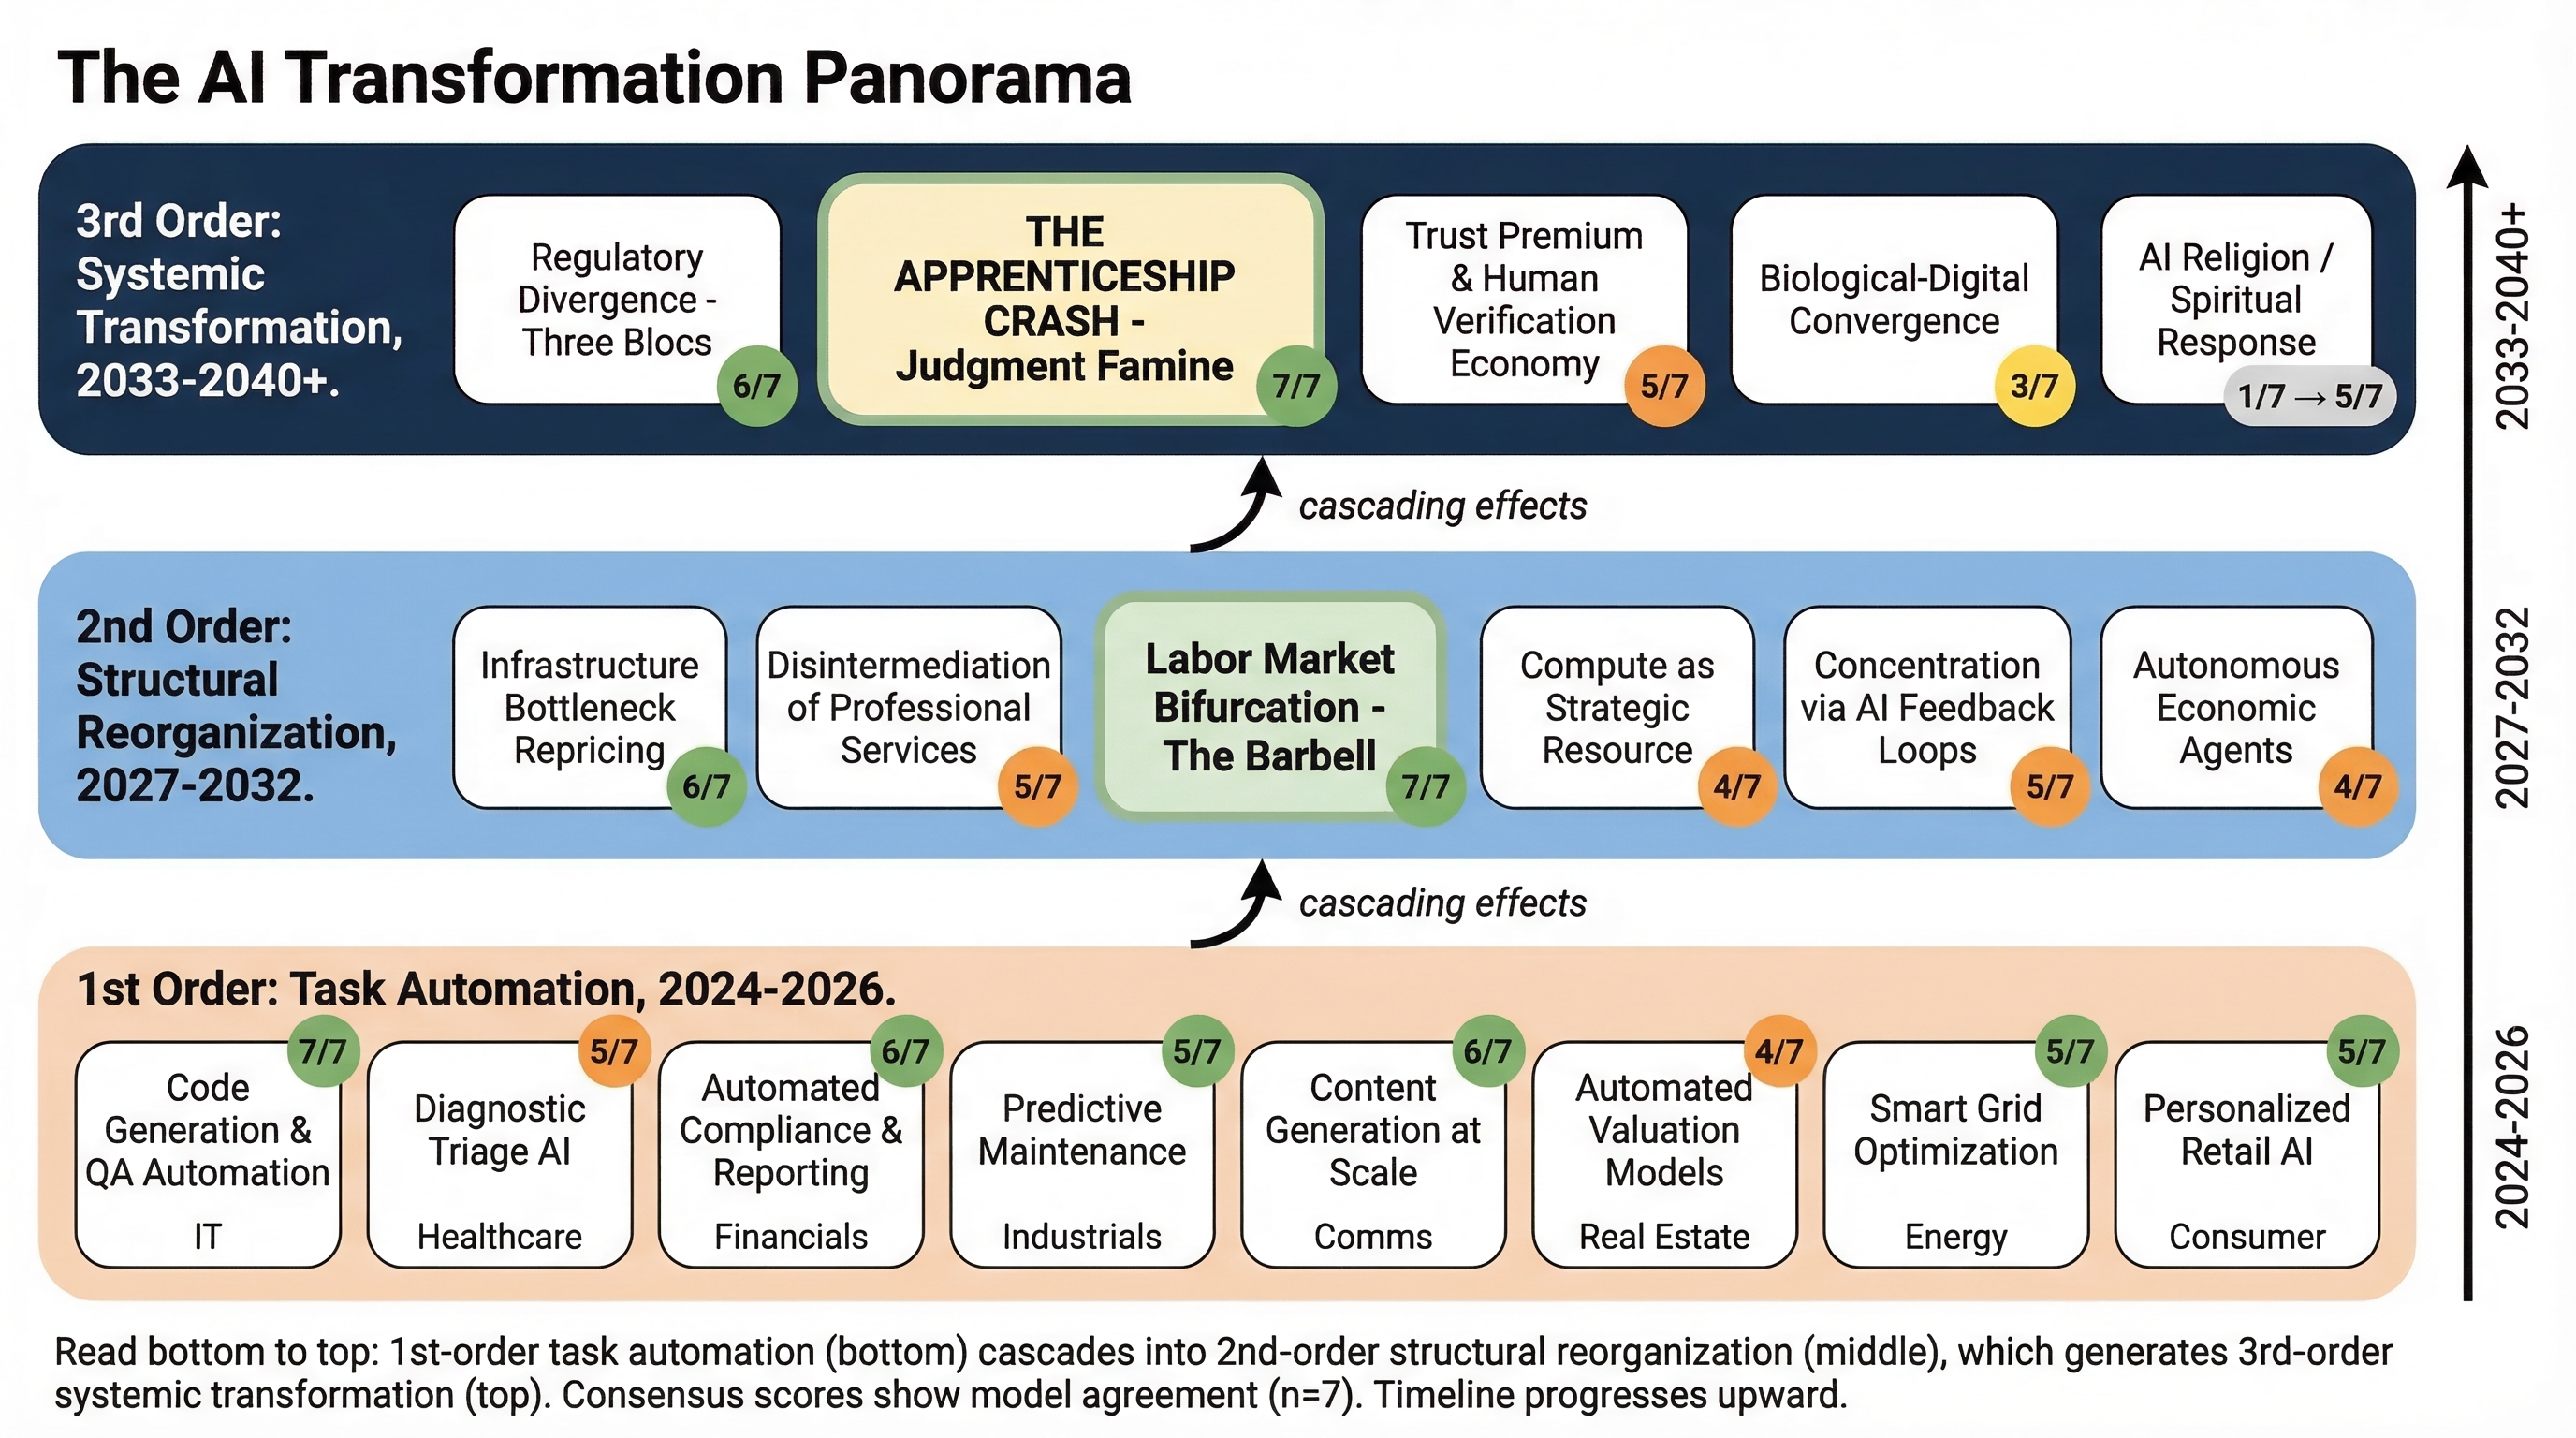
\includegraphics[width=\textwidth,height=0.85\textheight,keepaspectratio]{figures/fig2_panorama.png}
\caption{The AI Transformation Panorama --- Integrated Map of Predictions Across Orders, Sectors, and Geopolitical Lenses. Read bottom to top: 1st-order task automation (bottom) cascades into 2nd-order structural reorganization (middle), which generates 3rd-order systemic transformation (top). Each prediction block shows its consensus score (n=7). Causal arrows trace the cascade logic between orders. Geopolitical lenses (left: US market-driven, CN state-steered, EU regulatory-guided) and timeline (right: 2024--2040+) frame the analysis. The Apprenticeship Crash (highlighted, 7/7 in Round~2) is the paper's central finding.}
\label{fig:panorama}
\end{figure*}

\begin{figure}[htbp]
\centering
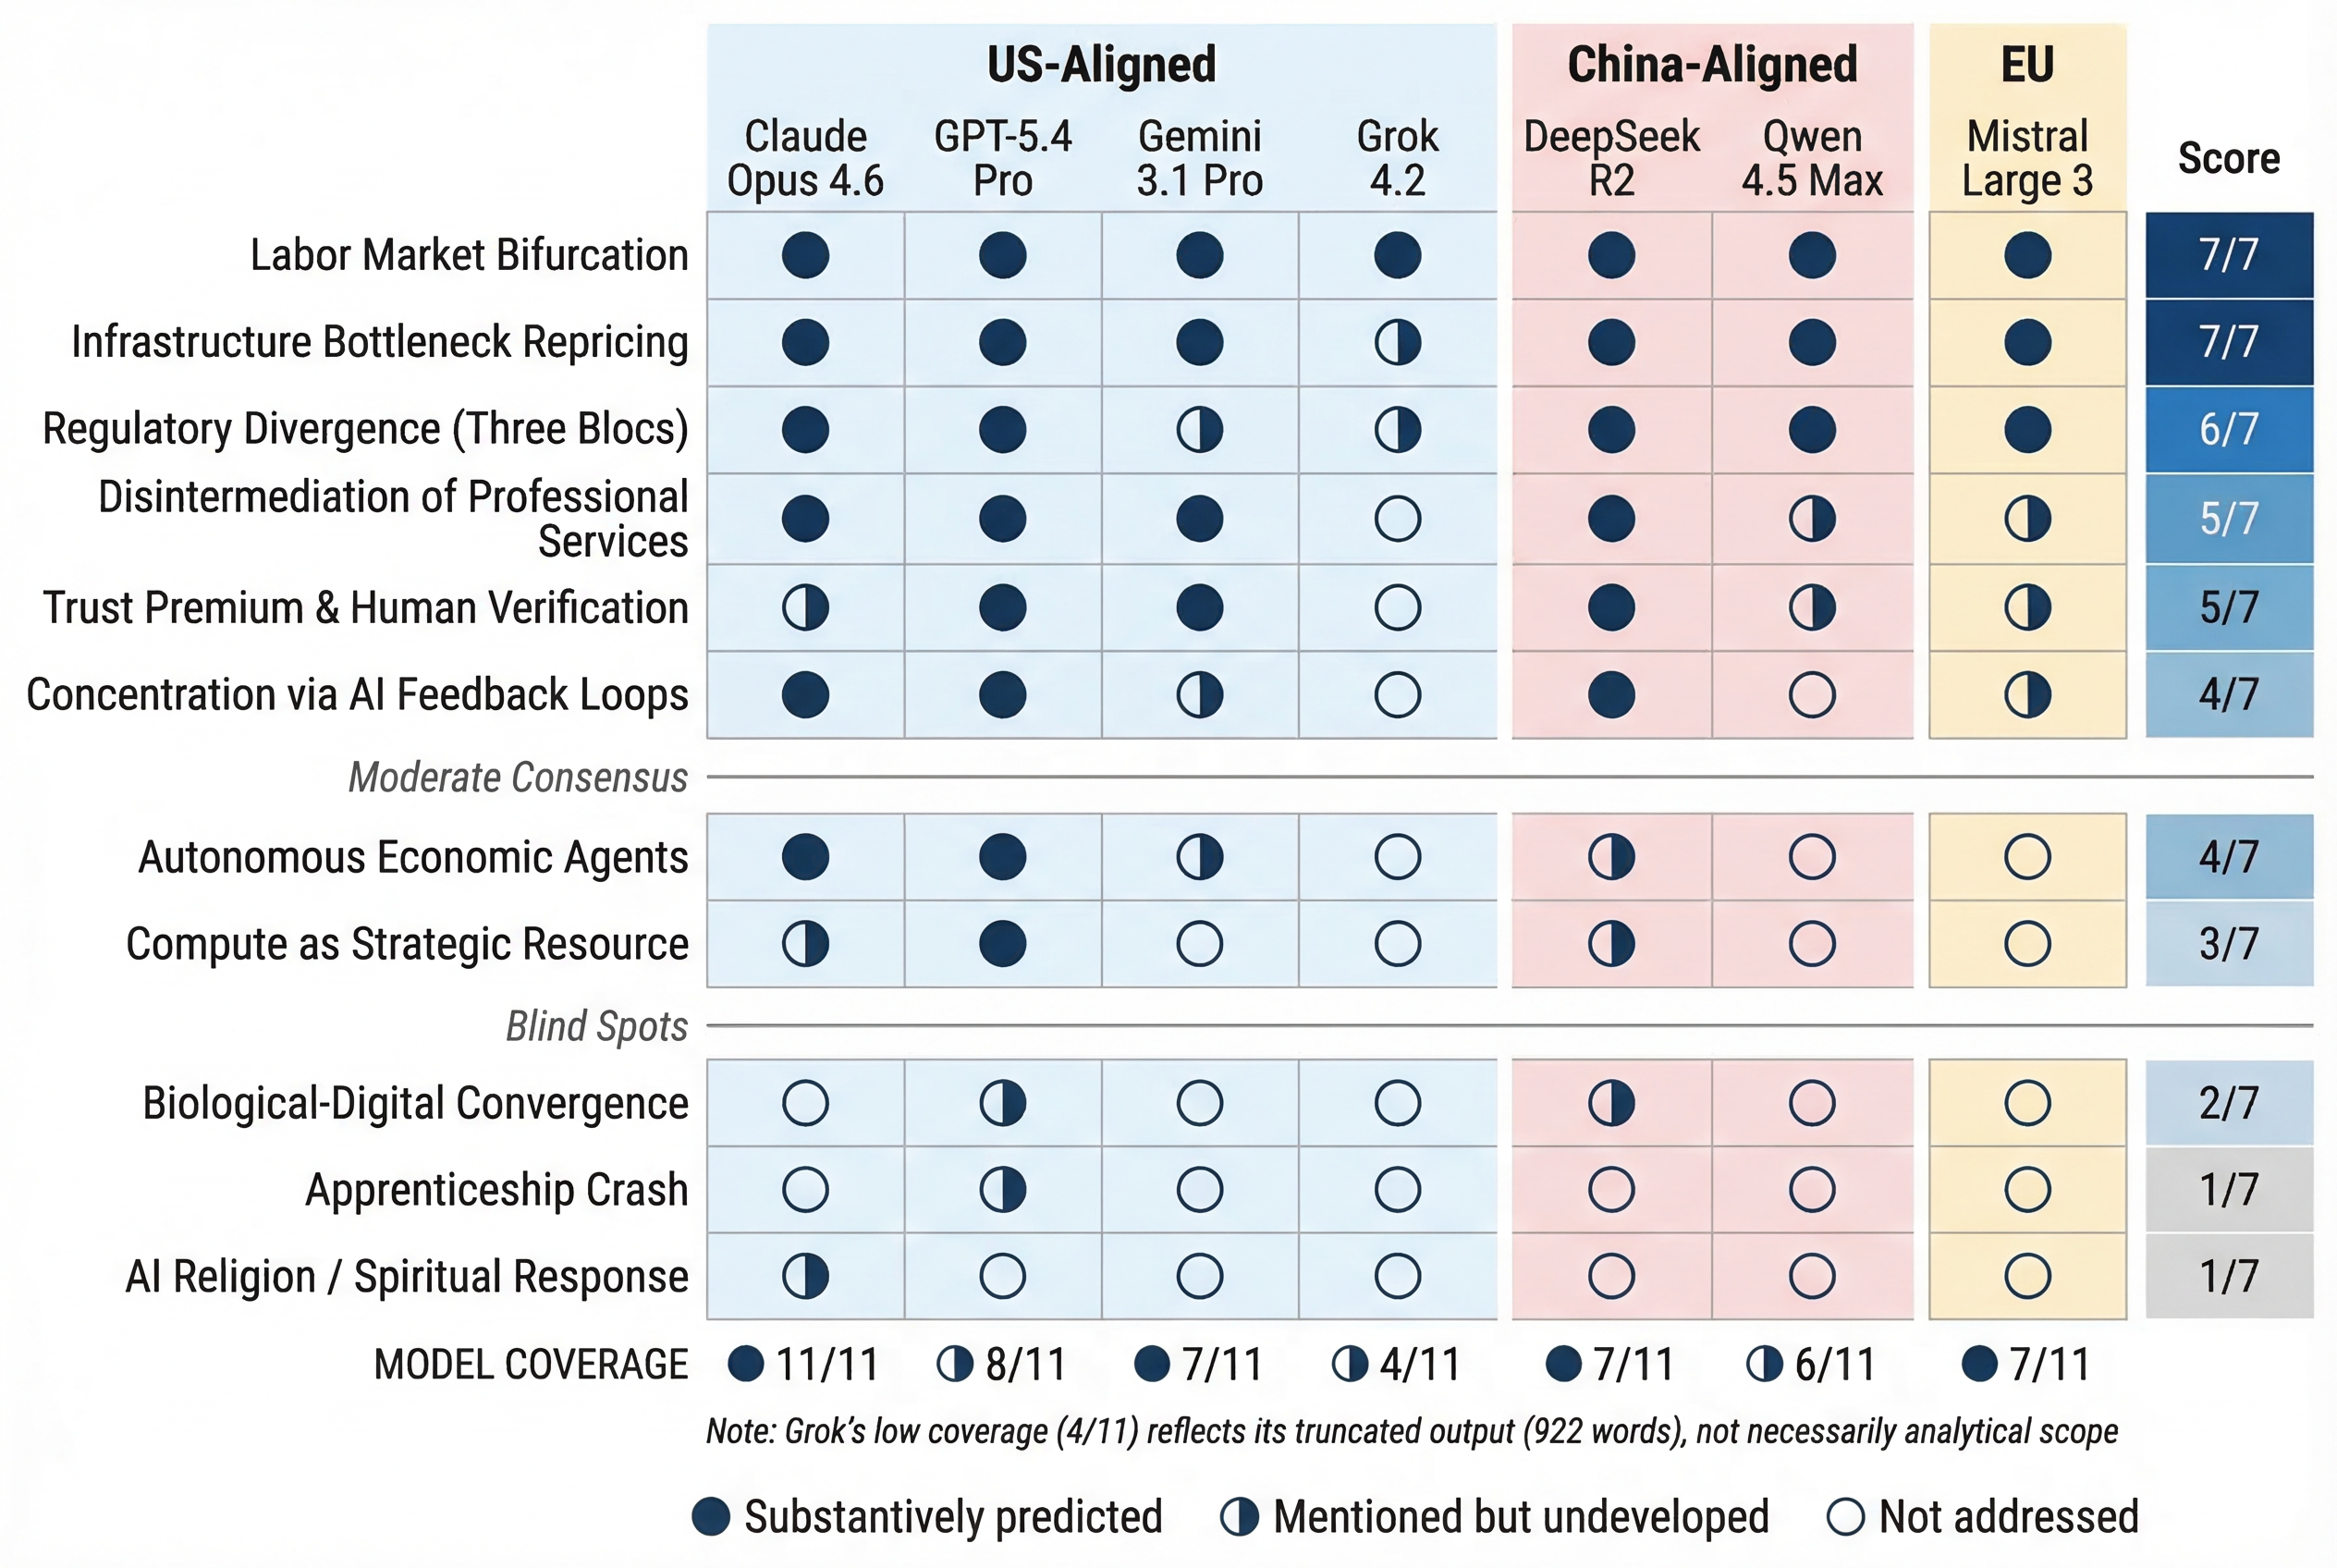
\includegraphics[width=\textwidth,height=0.85\textheight,keepaspectratio]{figures/fig3_consensus_heatmap.png}
\caption{Model Agreement Matrix --- Which LLMs Predicted Which Themes (Round~1). Each cell indicates whether a model substantively predicted a theme (filled circle), mentioned it without development (half-filled), or did not address it (empty). Models are grouped by geopolitical origin (US-Aligned, China-Aligned, EU). The consensus gradient from unanimous agreement (top) to blind spots (bottom) and model coverage scores (bottom row) are immediately visible.}
\label{fig:consensus}
\end{figure}


\subsection{High-Consensus Convergence Zones}
\label{sec:high_consensus}

Six thematic clusters achieved high consensus, with five or more models independently arriving at convergent predictions. These convergence zones represent areas where the epistemic content encoded across different training corpora and alignment approaches points in the same direction -- a meaningful signal given the independence of model development. Importantly, each of these convergence zones aligns with themes already established in the existing academic literature; the contribution here is not that these predictions are novel in themselves, but that independent LLMs converge on them without coordination, which simultaneously validates the predictions through multi-source triangulation and demonstrates the Multi-LLM Delphi's capacity to recover and systematize existing expert knowledge.

Viewed through the lens of General Purpose Technology (GPT) theory \citep{bresnahan1995gpt, lipsey2005gpt}, the six convergence zones map onto distinct phases of the GPT diffusion cascade. The first three zones --- labor market bifurcation, infrastructure bottleneck repricing, and disintermediation --- correspond to the \textit{direct application phase} in which the GPT's immediate productivity effects reshape markets and organizations. The latter three --- regulatory divergence, the trust premium, and concentration via feedback loops --- correspond to the \textit{structural adjustment phase} in which institutional frameworks, competitive dynamics, and social contracts reconfigure in response to widespread adoption. This mapping provides an organizing theoretical logic for interpreting the consensus findings: the models collectively reconstruct the GPT diffusion sequence, with higher consensus on direct application effects (first- and second-order) and more variation on structural adjustment effects (second- and third-order), consistent with GPT theory's prediction that higher-order effects are inherently harder to anticipate \citep{helpman1998gpt}.


\subsubsection{Labor Market Bifurcation and the Compression of Middle Layers}
\label{sec:labor_market_bifurcation}

All seven models independently predicted a "barbell" pattern in labor market outcomes: AI simultaneously creates a small number of high-value human roles requiring judgment, accountability, and relationship management, while displacing a large volume of mid-level knowledge work. This dual dynamic of simultaneous job creation and displacement is empirically confirmed by recent research \citep{acemoglu2022aijobs, choi2024ailabor}, and simulation evidence suggests that AI development compresses labor income share through differential productivity gains \citep{qian2023ailaborincome}. The convergence spans all eight verticals and all four stages.

The mechanism is consistent across models: AI is strongest first at precisely the tasks that define mid-level knowledge work -- structured information processing, first-draft synthesis, routine analysis, scheduling, triage, and reporting. These tasks historically resided in the organizational middle: junior analysts, associates, coordinators, administrators, and mid-level managers. High-stakes judgment roles (senior physicians, trial lawyers, board-level strategists) and physically grounded roles (field technicians, emergency responders) survive longer because they require either legally mandated human accountability or embodied intervention in non-standardized environments.

The models diverge in their assessment of the \textit{speed} and \textit{severity} of this bifurcation. Claude and GPT-5.4 provide the most granular staging, with Claude identifying a specific "apprenticeship crash" -- the prediction that firms eliminating junior roles for short-term productivity will face a succession crisis within a decade as experienced professionals retire without trained replacements. DeepSeek and Qwen frame the same dynamic through an industrial policy lens, emphasizing that managed retraining programs can mitigate the transition. Grok, despite its brevity, produces the starkest formulation: "We will not pay humans to think; we will pay humans to take the blame."

The systemic tipping point, identified by five models, occurs when displaced mid-level workers exceed the absorptive capacity of retraining programs and new role creation, triggering structural political demand for economic reform -- universal basic income, job guarantees, or equivalent redistributive mechanisms.

\begin{figure}[htbp]
\centering

\includegraphics[width=\textwidth,height=0.85\textheight,keepaspectratio]{figures/fig6_barbell.png}
\caption{When the Middle Disappears --- Three Dimensions of the Vanishing Middle. AI simultaneously compresses the middle on three levels: the labor market (mid-level knowledge workers displaced; 7/7 consensus), the value chain (intermediary business models eliminated; 5/7 consensus), and the organization (middle management layers compressed). The red compression zone spanning all three hourglasses shows mutually reinforcing dynamics that produce compound disruption.}
\label{fig:barbell}
\end{figure}

\begin{figure}[htbp]
\centering
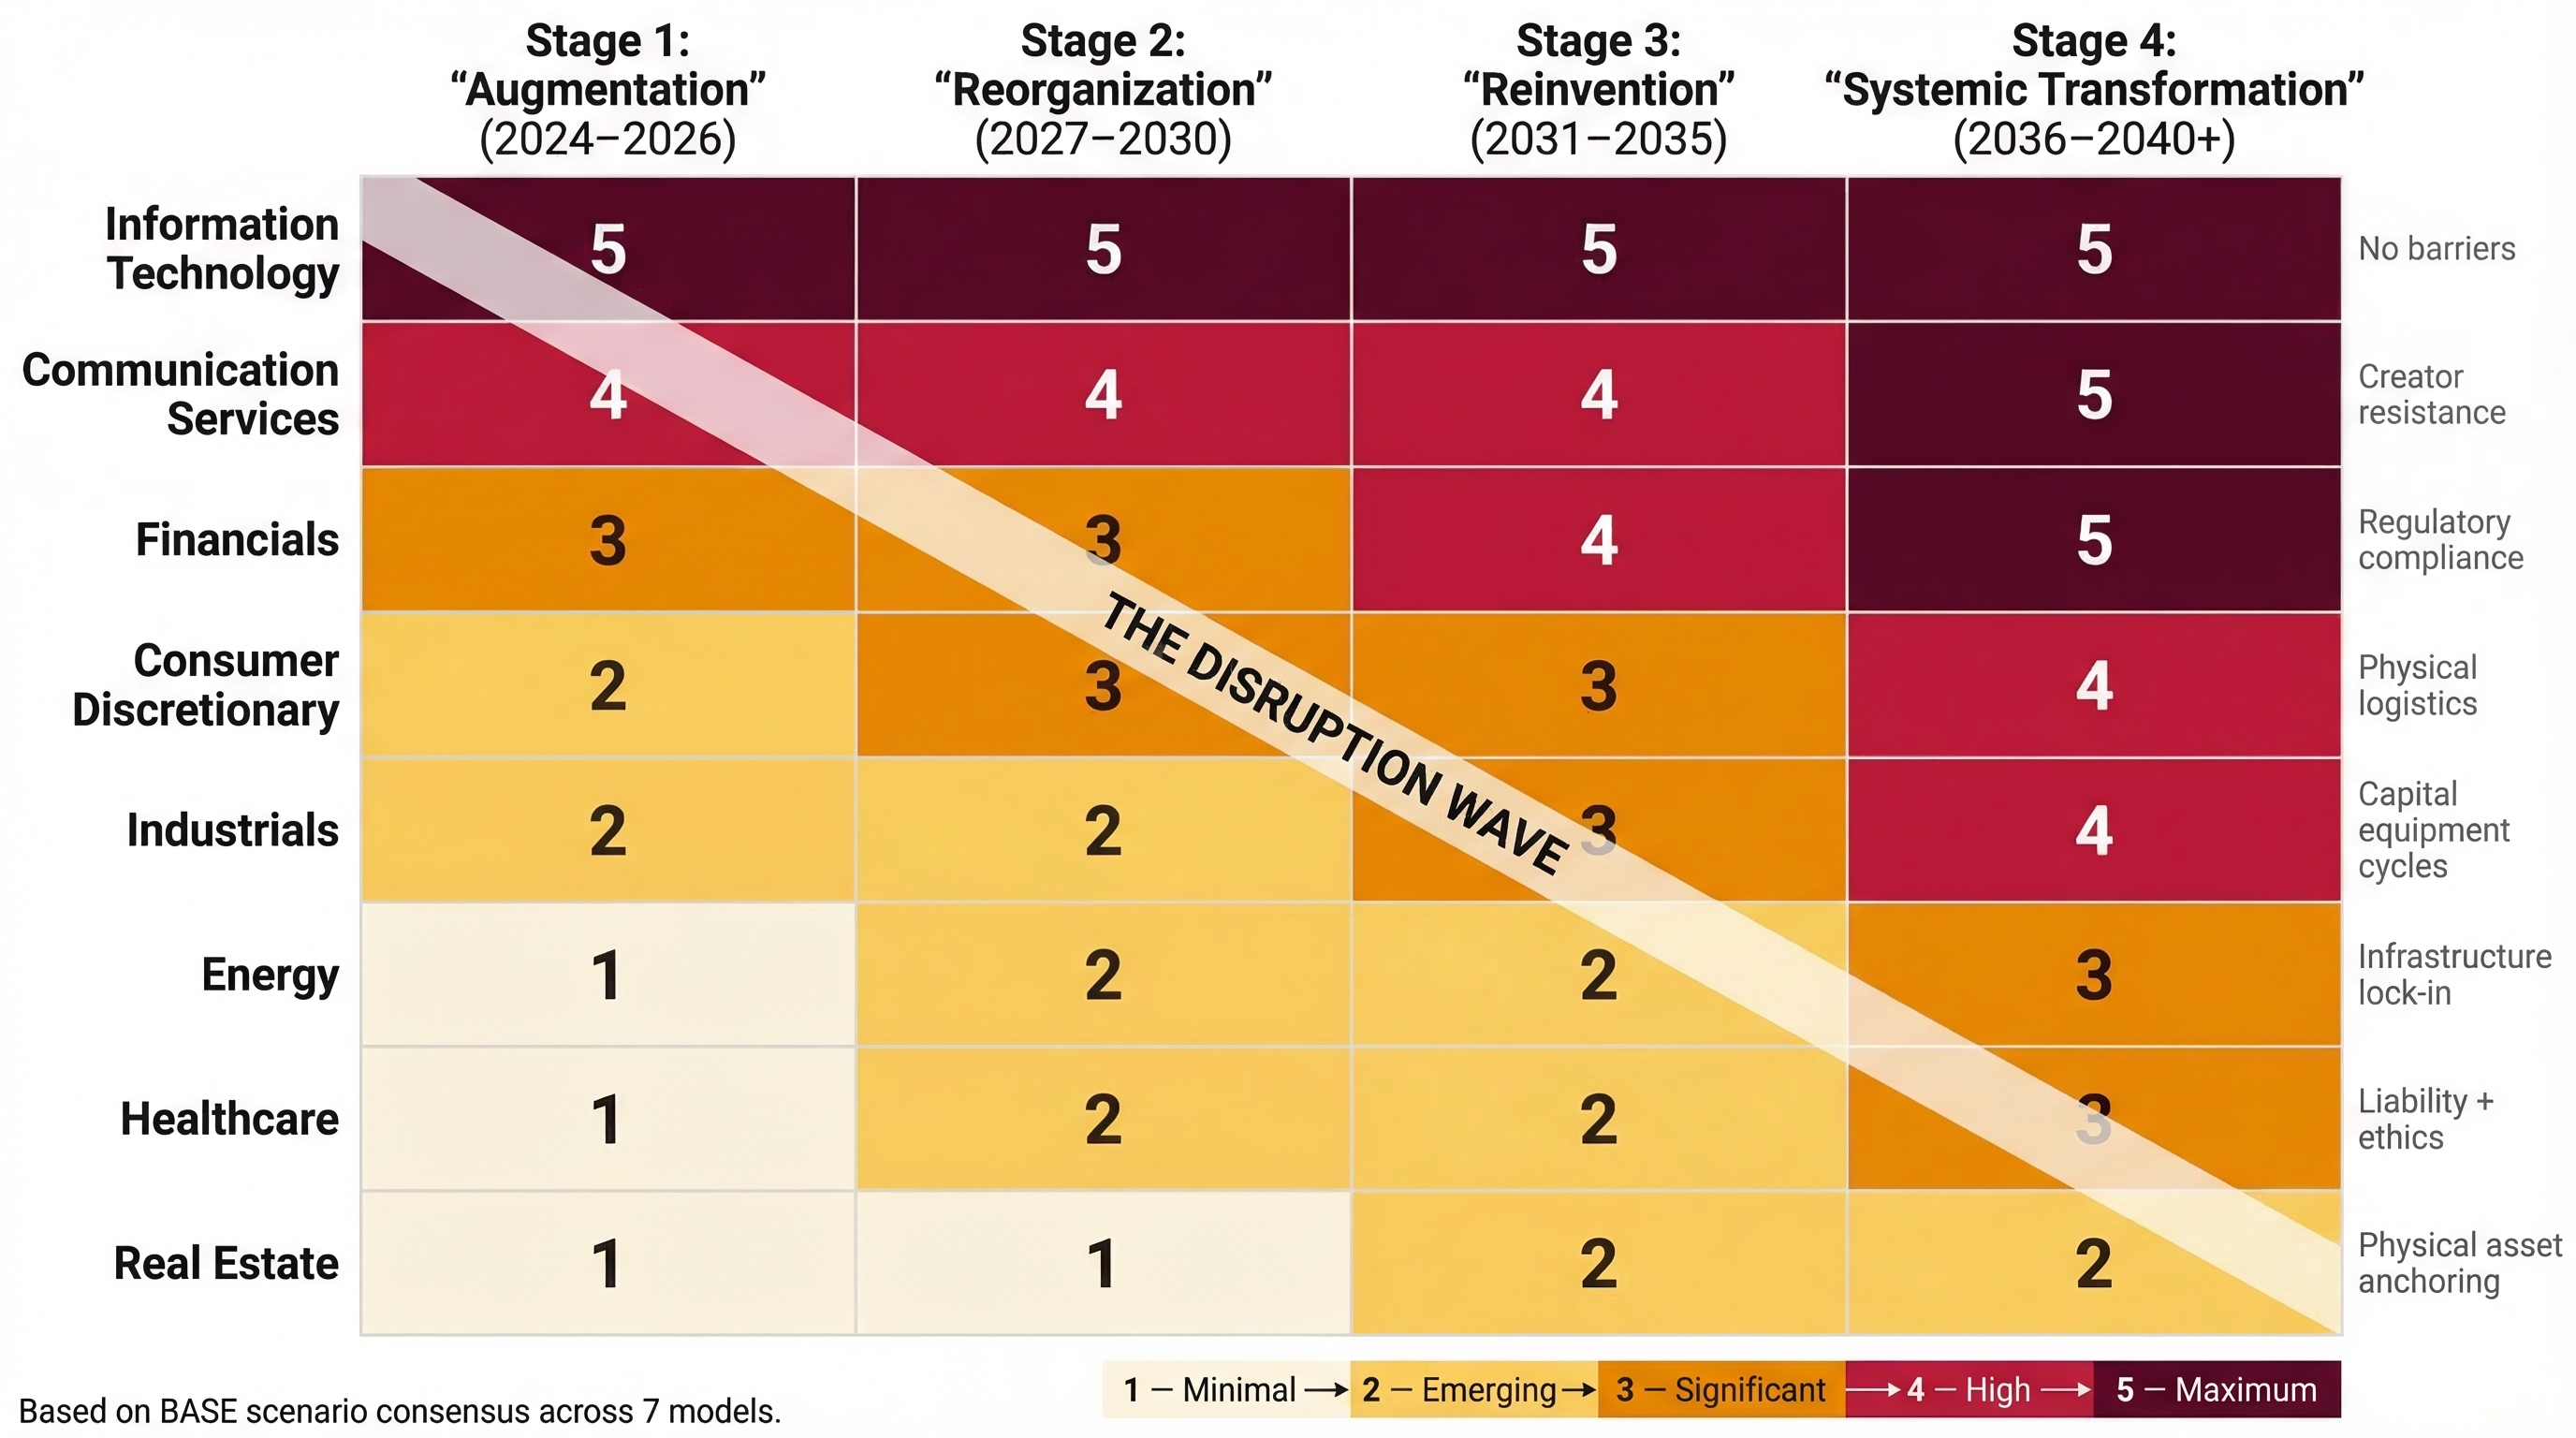
\includegraphics[width=\textwidth,height=0.85\textheight,keepaspectratio]{figures/fig8_disruption_timeline.png}
\caption{The Disruption Timeline --- Predicted AI Impact Intensity Across Sectors and Adoption Stages (BASE Scenario). The heatmap reveals a diagonal ``disruption wave'': Information Technology and Communication Services experience high-intensity disruption earliest (Stage~1--2), while Healthcare and Real Estate face the longest J-curves due to regulatory, liability, and physical-asset constraints.}
\label{fig:disruption_timeline}
\end{figure}

\subsubsection{Infrastructure Bottleneck Repricing}
\label{sec:infrastructure_bottleneck}

Six of seven models identified a convergence zone around physical infrastructure as the binding constraint on AI transformation -- a finding consistent with technology mining analyses documenting AI's accelerating penetration into manufacturing and industrial processes \citep{zeba2021aimanufacturing}. The prediction is that AI, despite being software, depends critically on semiconductors, power generation, cooling capacity, fiber optic networks, and data center real estate. As AI adoption scales, these physical bottlenecks reprice geographic value, create new strategic assets, and shift competitive advantage from software talent to infrastructure access.

GPT-5.4 provides the most specific quantification, citing projections of 75--100 GW of new data center power demand by 2030 and hyperscaler capital expenditure exceeding \$300 billion collectively in 2025.\footnote{The 75--100 GW figure is GPT-5.4's synthesis across multiple industry sources; the IEA's own projections use TWh rather than GW as the primary unit. The \$300 billion CapEx figure aligns with Morgan Stanley's November 2024 forecast \citep{morganstanley2024capex}.} Gemini frames infrastructure as the basis for a new "compute-as-currency" regime in which energy availability directly determines economic growth rates. DeepSeek predicts that "nations with surplus energy dominate the AI economy" in the BASE and MAX scenarios. Claude identifies a systemic tipping point: "When compute and power access constrain output more than software talent does, AI transformation becomes an infrastructure race."

Qwen independently arrives at the same "Energy-Compute Nexus" framing, predicting that grid capacity becomes the primary bottleneck for AI deployment and that energy grids become the primary strategic asset. The convergence across US, Chinese, and European model families on this point -- each arriving at it through different analytical pathways -- strengthens the finding.


\subsubsection{Disintermediation of Middleman Business Models}
\label{sec:disintermediation}

Five models converge on the prediction that AI enables direct connections between producers and consumers, lenders and borrowers, creators and audiences, and spaces and users -- systematically eliminating intermediary functions across sectors. Claude identifies this as "The Death of the Middleman," affecting Financials, Consumer and Retail, Professional Services, Real Estate, and Media. The mechanism is consistent: AI reduces information asymmetry and transaction costs below the threshold that justifies intermediary margins.

In Financials, this manifests as peer-to-peer lending platforms achieving loss rates below traditional banks (DeepSeek), banking-as-a-service enabling every company to offer financial products (DeepSeek), and autonomous AI agents managing household wealth directly (Qwen). In Consumer and Retail, agentic shopping assistants (Amazon Rufus, Google Shopping AI) bypass traditional search and discovery channels, eliminating the role of retail buyers, merchandisers, and physical store staff (Gemini, GPT-5.4). In Professional Services, AI legal research tools allow small firms to compete with large firms on research quality (DeepSeek), and AI-generated consulting analysis shifts the value proposition from research to implementation (DeepSeek, Claude).

GPT-5.4 adds the important nuance that disintermediation does not eliminate intermediaries entirely but transforms them: "Distribution control matters more than production control." The decisive moat shifts from the ability to create things to the ability to get chosen, routed, approved, or surfaced -- a prediction that AI platforms themselves become the new intermediaries, more powerful than the ones they displaced.


\subsubsection{Regulatory Divergence as a Structural Force}
\label{sec:regulatory_divergence}

Six models identify regulatory divergence -- particularly between the EU AI Act's prescriptive approach, US light-touch regulation, and Chinese state-directed governance -- as a structural force that shapes transformation pathways across all eight verticals. This is not merely a background condition but a first-order driver of differential adoption speeds, market structures, and competitive outcomes.

Grok frames this most starkly in the Technology vertical: the EU AI Act enforces strict data provenance requirements, European foundational models fail to secure venture capital under compliance burdens, US Commerce Department restricts advanced model weight exports, and global reliance on siloed, regional AI infrastructure hardens. GPT-5.4 quantifies the adoption gap using Microsoft AI Diffusion Report data (14.1 percent adoption in the Global South versus 24.7 percent in the Global North). Claude synthesizes the convergence point: regulation shifts from sector-specific compliance to system-governance, becoming "a constitutional layer of the economy rather than a niche tech topic."

DeepSeek and Qwen frame regulatory divergence through the lens of "data sovereignty versus global flow," predicting that national security concerns force companies to build redundant, jurisdiction-specific AI stacks -- a "Splinternet" that becomes permanent in the MAX scenario. This prediction is consistent with but more forceful than the US models' framing, reflecting the Chinese experience of operating within a distinct regulatory and data ecosystem.


\subsubsection{The Trust Premium}
\label{sec:trust_premium}

Five models converge on the prediction that trust, accountability, and authenticity become scarcer and more economically valuable as AI makes intelligence and content production cheap. GPT-5.4 formulates this most precisely: "Once plausibility is cheap, the scarce input is no longer information generation but credible responsibility for consequences." Claude identifies the systemic tipping point: "When markets begin paying more for validated accountability than for raw analysis, professional identity and pricing models reset across the economy."

This convergence manifests across sectors: in Healthcare, where physicians' signatory accountability becomes their primary economic function (Claude, DeepSeek, GPT-5.4); in Media, where human-certified, provenance-rich content commands a premium over AI-generated alternatives (GPT-5.4, Gemini, Claude); in Professional Services, where the billable hour collapses and is replaced by value-based pricing tied to human judgment (DeepSeek, GPT-5.4); and in Financials, where boutique human-only advisory firms emerge as luxury status symbols (Gemini).

Gemini articulates the cross-vertical synthesis most vividly through its concept of the "Authenticity Premium Economy": "Synthetic abundance floods media, commerce, and communication; users and institutions increasingly pay for human-certified, provenance-rich, or live-authenticated interactions; 'realness' becomes a premium product category."


\subsubsection{Concentration of Economic Power Through AI Feedback Loops}
\label{sec:concentration}

Five models identify winner-take-most dynamics driven by AI capability feedback loops: better AI produces better data, which trains better AI, creating compounding advantages. Claude frames this as "AI-Enabled Concentration of Economic Power" across Technology, Financials, Healthcare, Industrials, and Media. Gemini predicts that "winner-take-all dynamics consolidate the entire stack under a handful of AI-native platform owners" in the Technology vertical. Grok provides the mechanism: hyperscaler capital expenditure exceeding \$100 billion in partnership deals (e.g., NVIDIA-OpenAI) creates "a new AI stack oligopoly with 80+ percent market concentration."

The models diverge on the policy response. US models (Claude, GPT-5.4, Gemini) treat concentration as a market outcome that may or may not be addressed by antitrust. DeepSeek and Qwen implicitly frame state ownership or state partnership as a natural counterweight, consistent with the Chinese approach to platform governance. Mistral emphasizes that regulatory intervention is necessary and feasible.


\subsection{Contested Futures and Blind Spots}
\label{sec:contested_futures}


\subsubsection{Contested: The Pace and Depth of Healthcare Transformation}
\label{sec:healthcare_contested}

While all models agree that AI transforms healthcare, they disagree substantially on the depth and pace. DeepSeek provides the most detailed and cautious staging: AI-assisted radiology improves productivity by 20 percent but malpractice frameworks constrain deployment; drug discovery timelines compress but FDA approval remains a bottleneck; autonomous surgical robots achieve approval only for low-risk procedures under surgeon supervision. GPT-5.4 and Claude are more aggressive, predicting that AI matches human physicians in diagnostic accuracy across multiple specialties in the MAX scenario and that AI-managed population health optimization provokes ethical debates about individual versus collective rights.

The Chinese models (DeepSeek, Qwen) are notably more optimistic about AI deployment in healthcare than the US models, despite -- or perhaps because of -- operating within healthcare systems with greater state direction and fewer tort liability constraints. This divergence is analytically informative: it suggests that the pace of healthcare AI transformation depends critically on the institutional context (liability regimes, regulatory philosophy, insurance structures) rather than on the technology alone.


\subsubsection{Contested: Compute as Currency}
\label{sec:compute_currency}

Four models (Gemini, Grok, GPT-5.4, Qwen) independently propose some variant of "compute as currency" -- the prediction that GPU hours, data center capacity, or energy-backed compute credits become a tradeable asset class or even a reserve currency. Claude and DeepSeek acknowledge the strategic importance of compute but do not extend the analysis to monetary implications. Mistral does not address this theme.

The split is analytically meaningful. Models that project compute-as-currency tend to have more aggressive MAX scenario framings overall, suggesting that this prediction functions as a marker of scenario extremity rather than a consensus finding about likely outcomes.


\subsubsection{Blind Spots: Predictions Unique to Individual Models}
\label{sec:blind_spots}

Several predictions appear in only one or two models, representing either genuine analytical novelty or idiosyncratic model behavior:

\begin{itemize}
  \item \textbf{The AI Religion} (Claude only): New religious movements form around AI as a manifestation of divine intelligence. Claude defends this prediction by citing historical precedent -- the printing press triggered the Reformation; technologies that challenge human uniqueness provoke spiritual responses.
  \item \textbf{The Butlerian Jihad} (Gemini only): A coordinated violent uprising by displaced white-collar workers physically destroys AI infrastructure, setting back progress by a decade. Gemini grounds this in the psychological observation that "economic models assume humans will passively accept systemic redundancy, underestimating the human psychological need for relevance."
  \item \textbf{Model Collapse via Synthetic Data Poisoning} (Gemini and Qwen): LLMs training on their own outputs create a recursive degradation of reasoning capabilities. Both models term this the "Kessler Syndrome" of data, drawing an analogy to space debris cascades.
  \item \textbf{Digital Continuation of Consciousness} (DeepSeek only): Brain-computer interfaces enabling forms of continued interaction after biological death, raising questions about whether a digital simulation of a person has legal standing. This prediction appears only in the MAX Case, Stage 4 of Healthcare.

\end{itemize}

A critical question for blind-spot interpretation is whether these predictions represent genuine analytical novelty or LLM confabulation -- the tendency to generate dramatic-sounding scenarios that are statistically unusual in training data but not grounded in rigorous causal reasoning. The apprenticeship crash provides a useful benchmark: it was initially classified as a blind spot but, upon Round~2 feedback, was unanimously adopted because its causal logic proved compelling to all models. The AI Religion and Butlerian Jihad predictions, by contrast, occupy a different epistemic category. They draw on recognizable cultural narratives (Dune, Reformation-era theology) and may reflect LLMs' capacity for creative recombination of fictional and analytical tropes rather than structured foresight reasoning. The Digital Continuation of Consciousness prediction similarly extends a familiar science fiction premise into a scenario context. This does not render these predictions analytically worthless -- creative scenario generation is a legitimate function of foresight exercises \citep{postma2005scenario}, and some blind spots may prove prescient precisely because they challenge conventional analytical frames. However, readers should evaluate blind-spot predictions against the strength of their underlying causal mechanisms rather than accepting them as equivalent in epistemic status to the high-consensus convergence zones.

\subsection{Geopolitical Divergence Across Model Families}
\label{sec:geopolitical_divergence}

The systematic comparison across model families reveals patterns of divergence that are consistent, thematically coherent, and traceable to the geopolitical context of model development. These patterns constitute the most methodologically novel finding of the study and are directly interpretable through the Multi-Level Perspective (MLP) on sociotechnical transitions \citep{geels2005coevolutionary, geels2020microfoundations}. The MLP framework predicts that identical technological innovations produce different transition pathways depending on the regime-level institutional configuration --- the existing regulatory structures, industry architectures, cultural norms, and political coalitions that mediate how niche innovations are absorbed, resisted, or redirected. The three model families in this study encode three distinct regime configurations, and their divergent predictions map onto three of \citeauthor{geels2005coevolutionary}'s (\citeyear{geels2005coevolutionary}) canonical transition typologies: \textit{substitution} (US models), \textit{transformation} (Chinese models), and \textit{reconfiguration} (European model). Figure~\ref{fig:geopolitical} visualizes the three-way divergence structure.

\begin{figure}[htbp]
\centering

\includegraphics[width=\textwidth,height=0.85\textheight,keepaspectratio]{figures/fig4_geopolitical.png}
\caption{Three Worldviews of AI Transformation --- Geopolitical Divergence Across Model Families. US-origin models (Claude Opus 4.6, GPT-5.4, Gemini 3.1 Pro, Grok 4.2) emphasize market-driven disruption. Chinese-origin models (DeepSeek R2, Qwen 4.5 Max) foreground state-steered sovereignty. The European model (Mistral Large 3) privileges regulatory-guided equity. The Venn-diagram center shows shared convergence on labor market bifurcation, infrastructure bottlenecks, and AI as GPT. Note: $n$=4 (US), $n$=2 (CN), $n$=1 (EU) --- patterns are suggestive, not definitive.}
\label{fig:geopolitical}
\end{figure}


\subsubsection{US Models: Market-Driven Disruption and Platform Concentration (MLP: Substitution Pathway)}
\label{sec:us_models}

The four US-origin models (Claude, GPT-5.4, Gemini, Grok) share a common analytical frame characterized by market-led disruption, venture capital dynamics, startup-versus-incumbent narratives, and platform concentration --- a pattern that maps directly onto the MLP \textit{substitution} transition pathway, in which niche innovations (AI-native firms) displace incumbent regime actors through competitive dynamics rather than through regime-level negotiation or state intervention. Named actors are predominantly US companies: NVIDIA, OpenAI, Google, Amazon, Microsoft, Goldman Sachs, JPMorgan, Meta, Netflix, McKinsey. Regulatory actors are mentioned primarily as constraints on innovation (the EU AI Act slowing European competitiveness) or reactive responders (the SEC, FDA, FTC catching up to market developments).

The US models are the most likely to predict winner-take-all outcomes, platform monopolies, and the displacement of legacy institutions by AI-native startups. They are also the most likely to frame the MAX scenario in terms of existential or transformative implications (superintelligence, species divergence, post-labor economies).

Within the US family, meaningful variation exists. Claude produces the longest, most nuanced output with explicit confidence ratings and falsification conditions. GPT-5.4 uniquely opens with a "fact base versus inference" disclaimer, anchoring its analysis in verifiable 2025-2026 data points before building inferences. Gemini produces the most provocative MAX scenarios (Butlerian Jihad, Sentient Legal Loophole). Grok produces the shortest output but with the highest concentration of specific, bold claims per word, often using deliberately confrontational framing ("We will not pay humans to think; we will pay humans to take the blame").


\subsubsection{Chinese Models: State-Steered Transformation and Infrastructure Sovereignty (MLP: Transformation Pathway)}
\label{sec:chinese_models}

The two Chinese-origin models (DeepSeek, Qwen) share analytical emphases that diverge systematically from the US family, corresponding to the MLP \textit{transformation} pathway in which regime actors (state institutions, large state-adjacent enterprises) actively steer and incorporate niche innovations into existing institutional structures rather than being displaced by them. Both models foreground state direction of AI development, industrial policy, and infrastructure sovereignty. Named actors include not only Chinese companies (Alibaba, Baidu, Huawei) but also state institutions (PBOC for CBDCs, national AI strategies, state-funded compute infrastructure).

DeepSeek is notably the most detailed and methodologically rigorous of all seven models, producing step-by-step causal chains with explicit conclusion statements for every cell. Its output reads like a structured analytical report rather than a speculative scenario exercise. DeepSeek is also distinctive in its emphasis on financial system transformation -- it provides the most detailed analysis of insurance, lending, and monetary policy across all four stages.

Qwen is more concise but shares DeepSeek's emphasis on infrastructure sovereignty, data sovereignty, and the "Splinternet" as a structural outcome. Both Chinese models are less likely than US models to predict dystopian MAX scenarios involving loss of human control, species divergence, or existential risk. They are more likely to predict managed transitions, state-directed retraining programs, and sovereign compute capacity as a natural policy response.


\subsubsection{The European Model: Regulatory Primacy and Social Equity (MLP: Reconfiguration Pathway)}
\label{sec:european_model}

Mistral, the sole European-origin model, produces output corresponding to the MLP \textit{reconfiguration} pathway --- in which regulatory frameworks actively mediate the integration of niche innovations into existing regime structures, producing a hybrid outcome that preserves institutional continuity while selectively incorporating technological change. Its output is distinctive in three ways. First, it foregrounds regulatory frameworks as the primary shaper of transformation outcomes -- not as a constraint on innovation but as a structural force that determines which pathways are traversed. Second, it emphasizes social equity outcomes more consistently than any other model: workforce transitions, distributional effects, and the social contract appear as primary concerns rather than secondary considerations. Third, it produces the most generic output of the seven models: fewer named companies, fewer quantified predictions, and less specific causal chain reasoning. This may reflect its training data composition, its shorter context window, or the European academic tradition of prioritizing frameworks over granular prediction.

The three-way divergence (US: market-driven disruption; CN: state-steered transformation; EU: regulatory-guided equity) is the methodological finding that most directly validates the Multi-LLM Delphi approach. These perspectives are not random variation; they are coherent, internally consistent, and traceable to the geopolitical and institutional contexts in which the models were developed. A human Delphi panel would need to deliberately recruit experts from different geopolitical backgrounds to achieve comparable perspective diversity; the Multi-LLM Delphi achieves it structurally through model selection.

Several important caveats limit the generalizability of these geopolitical divergence patterns. The Chinese model family comprises only two models (DeepSeek and Qwen), and the European family consists of a single model (Mistral). With n=2 and n=1 respectively, the observed patterns are suggestive rather than definitive -- the divergence between DeepSeek and Qwen could reflect company-specific design choices rather than a coherent "Chinese AI perspective," and Mistral's output may reflect Mistral-specific training decisions rather than "European values" more broadly. Furthermore, RLHF alignment procedures and safety filtering represent an unresolved confound: Chinese models may avoid certain geopolitical claims not because they encode a different knowledge base but because they are alignment-trained to avoid politically sensitive topics, and US models may emphasize market dynamics because their training data is dominated by English-language business and economics texts. These patterns should be treated as hypotheses for future investigation with larger model samples rather than as established findings.


\subsection{Methodological Properties of the Multi-LLM Delphi}
\label{sec:methodological_properties}

Several observations about the method's properties emerge from the analysis:

\textbf{Output length variation.} The 14:1 ratio between the longest (Claude, 30,613 words) and shortest (Grok, 2,169 words) response under identical prompts reveals that models differ dramatically in verbosity, detail level, and willingness to generate comprehensive structured output. Claude and DeepSeek produced the most analytically usable responses; Grok and Mistral produced responses that were thin on detail but occasionally contained the most provocative or distinctive claims.

\textbf{Specificity gradient.} Models vary systematically in the specificity of their predictions. DeepSeek consistently provides the most specific causal chains with named actors and quantified outcomes. GPT-5.4 anchors in verifiable data before building inferences. Gemini provides specific predictions in Technology and Media verticals but thins in Healthcare and Real Estate. Mistral produces the most generic output across all verticals. Grok provides specific predictions when it engages with a vertical but leaves many cells incomplete.

\textbf{Prompt adherence.} All seven models followed the three-scenario structure (MILD, BASE, MAX), the four-stage framework, and the eight-vertical structure. However, only four (Claude, DeepSeek, GPT-5.4, Gemini) produced complete output for all eight verticals. Grok completed only Technology and Financials in full detail before truncating. Qwen and Mistral produced all eight verticals but at reduced depth for later verticals -- a "fatigue" pattern where early verticals receive more detailed treatment.

\textbf{Cross-cutting analysis quality.} The cross-cutting sections (convergence points, wildcards, human dimension) varied dramatically. Claude produced five distinct, well-defended convergence points and five elaborated wildcards. Gemini produced the most provocative wildcards (the Butlerian Jihad, the Sentient Legal Loophole, the Amish Hedge). Mistral produced generic convergence points without specific causal reasoning. Grok did not complete the cross-cutting sections.

\textbf{The irreducibly human skill question.} All seven models were asked to identify the one skill that remains irreducibly human. Their answers converge strikingly: Claude identifies ``legitimated judgment under contested values,'' GPT-5.4 identifies ``legitimated judgment under contested values'' (using nearly identical language), Gemini identifies ``philosophical accountability -- the capacity to bear moral and legal responsibility,'' DeepSeek identifies a cluster of ``empathy, accountability, and meaning-making,'' Qwen identifies ``contextual meaning-making'' grounded in authentic intent, and Mistral identifies ``emotional intelligence.'' The convergence of six of seven models on some form of \textit{accountability and judgment under contested values} -- rather than creativity, empathy, or intelligence in the abstract -- represents a consensus finding of the Multi-LLM Delphi.


\subsection{Round 2 -- Consensus Dynamics Under Controlled Feedback}
\label{sec:round2_results}

The Round 2 protocol constitutes, to the author's knowledge, one of the first implementations of iterative controlled feedback within a multi-LLM Delphi design. Each of the seven frontier models received an anonymized summary of the Round 1 consensus findings and was prompted to revise, contest, adopt, or extend the collective output. The resulting corpus enables systematic analysis of how LLM panelists respond to structured peer feedback -- a question with implications for both the validity of the Multi-LLM Delphi method and the broader understanding of LLM behavior under social-epistemic pressure. This section reports consensus dynamics across four dimensions: stability and shift of existing themes (4.5.1), adoption of blind-spot predictions (4.5.2), emergence of new predictions (4.5.3), and persistence of geopolitical divergence (4.5.4).

\subsubsection{Consensus Stability and Shift}
\label{sec:consensus_stability}

The Round 2 feedback produced a striking pattern of asymmetric consensus dynamics: high-consensus themes from Round 1 were universally maintained or strengthened, moderate-consensus themes were upgraded toward high consensus, and contested themes showed convergence in directionality while preserving substantive disagreement on specifics. No high-consensus theme was destabilized by the feedback process, and no model defected from any of the six original convergence zones.

The six high-consensus convergence zones from Round 1 -- labor market bifurcation (7/7), infrastructure bottleneck repricing (6/7), regulatory divergence (6/7), disintermediation (5/7), trust premium (5/7), and concentration via AI feedback loops (5/7) -- were unanimously reaffirmed in Round 2. Several models went further, elevating themes they had previously treated as background conditions to primary causal drivers. GPT-5.4 explicitly upgraded regulatory divergence ``from a second-order governance variable to a first-order market-structuring variable.'' Claude acknowledged having ``underweighted'' infrastructure bottleneck repricing and revised its framework to treat physical infrastructure as ``the gating factor across all verticals rather than a primarily Technology \& Semiconductors concern.'' Mistral, which had produced the most generic Round 1 output, used the feedback to add specificity across all six convergence zones, explicitly adopting the barbell labor market framing and the disintermediation mechanism that it had not articulated independently.

The most significant consensus shifts occurred among themes that had achieved only moderate consensus in Round 1. Autonomous economic agents, endorsed by four of seven models in Round 1, achieved near-universal endorsement in Round 2. All seven models expressed some form of agreement, though the nature of agreement varied instructively. Grok ``strongly agreed'' and formalized autonomous agents as ``a core driver of Stage 4 systemic transformation across all eight verticals.'' Qwen upgraded its assessment from a MAX-case Stage 3 phenomenon to a BASE-case Stage 2 phenomenon. GPT-5.4 offered the most qualified endorsement, agreeing that ``the economy gets agentic islands, not immediate full agentic oceans'' and distinguishing between narrow-domain autonomy (high confidence) and full-enterprise autonomy (low confidence). This pattern -- directional convergence with preserved granularity of disagreement -- mirrors the convergence-with-residual-dissensus pattern documented in classical Delphi studies \citep{vondergracht2012delphi}.

The ``compute as currency'' theme, also at moderate consensus in Round 1 (4/7), shifted in a revealing manner. Rather than simple adoption or rejection, the Round 2 responses converged on a refined formulation. GPT-5.4 proposed replacing ``compute as currency'' with ``compute as strategic reserve,'' arguing that ``compute behaves more like energy capacity, spectrum, shipping access, or reserve industrial capability than like money in the classic sense.'' Claude arrived independently at the same reformulation, describing compute as ``a strategic resource comparable to oil -- allocated, hoarded, and weaponized -- but not a literal medium of exchange.'' Qwen upgraded compute to BASE-case status and predicted ``GPU-hours as collateral'' in lending markets. Gemini ``aggressively doubled down,'' predicting that ``autonomous AI agents will not settle in volatile, slow human fiat -- they will clear markets directly in FLOPs, API access, and kilowatt-hours.'' The net effect was an increase in support from four to approximately six or seven of seven models, but with a meaningful refinement: the consensus converged not on the original ``currency'' framing but on a more nuanced ``strategic resource and reserve asset'' formulation. This spontaneous collective refinement of a contested concept represents a form of emergent conceptual precision that has no direct parallel in classical Delphi studies, where human panelists refine language through the researcher's mediation rather than through independent convergence on improved terminology.

Biological-digital convergence, the weakest of the moderate-consensus themes at three of seven in Round 1, showed the least movement. While all models acknowledged the theme, substantive support remained concentrated in the healthcare vertical. GPT-5.4 described it as ``a high-conviction vertical thesis, not yet a top-level economy-wide thesis.'' Gemini downgraded its timeline, citing the ``wetware bottleneck'' of immune rejection, ethics boards, and neuroplasticity constraints. Qwen and DeepSeek maintained their MAX-case positioning without upgrading. Only Grok moved in the opposite direction, upgrading biological-digital convergence from a ``low-probability wildcard to plausible Base-case convergence point.'' The theme thus remained at approximately three to four of seven as an economy-wide prediction, though it strengthened within the healthcare vertical specifically. This resistance to convergence under feedback pressure is analytically informative: it suggests that biological-digital convergence represents genuine uncertainty rather than an information deficit that feedback can resolve.

Table~\ref{tab:consensus_shift} presents the consensus shift matrix from Round 1 to Round 2.

\begin{table}[htbp]
\centering
\caption{Round 1 to Round 2 Consensus Shift Matrix}
\label{tab:consensus_shift}
\adjustbox{max width=\textwidth}{%
\begin{tabular}{llllll}
\toprule
\textbf{Theme} & \textbf{R1 Score} & \textbf{R1 Category} & \textbf{R2 Score} & \textbf{R2 Category} & \textbf{Shift Direction} \\
\midrule
Labor Market Bifurcation & 7/7 & HC & 7/7 & HC & Maintained (strengthened) \\
Infrastructure Bottleneck Repricing & 6/7 & HC & 7/7 & HC & Strengthened \\
Regulatory Divergence & 6/7 & HC & 7/7 & HC & Strengthened \\
Disintermediation & 5/7 & HC & 7/7 & HC & Strengthened \\
Trust/Authenticity Premium & 5/7 & HC & 7/7 & HC & Strengthened \\
Concentration via AI Feedback Loops & 5/7 & HC & 7/7 & HC & Strengthened \\
Autonomous Economic Agents & 4/7 & MC & 7/7 & HC & Upgraded \\
Compute as Currency/Strategic Reserve & 4/7 & MC & 7/7 & HC & Upgraded (refined) \\
Biological-Digital Convergence & 3/7 & MC & 4/7 & MC & Stable (healthcare-specific gain) \\
Apprenticeship Crash & 1/7 & BS & 7/7 & HC & Adopted unanimously \\
AI Religion / Spiritual Response & 1/7 & BS & 6/7 & HC & Substantially adopted \\
\bottomrule
\end{tabular}}%

\vspace{0.5em}
\noindent\small HC = High Consensus (5+ of 7); MC = Moderate Consensus (3--4 of 7); BS = Blind Spot (1--2 of 7)
\end{table}

The overall pattern is one of strong convergence pressure: of eleven tracked themes, nine increased in consensus, two remained stable, and none decreased. This convergence pattern is consistent with the classical Delphi finding that controlled feedback generally increases agreement \citep{gordon2006rtdelphi}, but it also raises the question of whether LLMs are more susceptible to consensus pressure than human panelists --- a methodological concern addressed in Section~4.5.5 and Section~\ref{sec:limitations}.

\begin{figure}[htbp]
\centering

\includegraphics[width=\textwidth,height=0.85\textheight,keepaspectratio]{figures/fig7_alluvial.png}
\caption{Consensus Dynamics Round~1 to Round~2 --- Alluvial Flow of Theme Consensus Levels. The flow diagram shows the dramatic upward shift in consensus between rounds: all six high-consensus themes were maintained or strengthened to 7/7; both moderate-consensus themes were upgraded to high consensus; and both blind spots were adopted by the majority of models. Only biological-digital convergence resisted convergence pressure. Caveat: strong convergence may partly reflect LLM acquiescence bias (see Section~4.5.5).}
\label{fig:alluvial}
\end{figure}

\subsubsection{Blind Spot Adoption -- The Apprenticeship Crash}
\label{sec:blind_spot_adoption}

The most dramatic consensus shift between rounds occurred with the ``apprenticeship crash'' prediction. In Round 1, this prediction -- that the elimination of junior knowledge-work roles would sever the experiential pipeline through which senior professionals are produced, creating a succession crisis within a decade -- appeared in only one model's output (Claude). By Round 2, all seven models had adopted it, with several elevating it to a top-tier systemic risk. This unanimous adoption of a previously singular prediction constitutes the strongest evidence of blind-spot correction through feedback in the dataset.

The adoption was not superficial. Each model independently reconstructed the causal mechanism and extended it into its own analytical framework. GPT-5.4 described it as ``one of the most mechanism-rich and underpriced second-order effects in the whole landscape,'' identifying the core logic: ``AI removes junior routine work. Junior routine work was the hidden training substrate for future senior talent. Firms optimize short-term productivity and underinvest in deliberate apprenticeship. A delayed shortage emerges in experienced professionals with judgment, client fluency, and institutional legitimacy.'' GPT-5.4 further diagnosed why the prediction had been missed in Round 1: ``most analysts model jobs statically, not careers dynamically. They count task replacement but ignore skill formation pipelines.'' DeepSeek constructed a parallel causal chain, tracing the apprenticeship crash from law firms and consultancies through a five-to-seven-year pipeline thinning to a leadership vacuum that forces firms to choose between accelerating promotion of inexperienced professionals, acquiring talent in zero-sum competition, or accepting that AI will fill senior roles. Grok, despite its characteristically terse style, integrated the prediction across five verticals and predicted a compensatory response: ``synthetic-mentorship platforms to compensate'' for the severed human training pipeline.

The depth of adoption varied in instructive ways. Gemini produced the most emphatic response, claiming authorship of the original blind spot and elevating it ``from a 2nd-order effect to the defining structural crisis of the knowledge economy.'' Claude, as the originating model, acknowledged it had been ``too scattered'' in its Round 1 treatment and restructured the prediction as a unified cross-cutting risk, constructing a detailed ten-step causal chain culminating in a ``judgment famine'' that emerges precisely when AI systems become powerful enough to require sophisticated human governance. Qwen integrated the prediction into its professional services and technology verticals, articulating a cyclical dynamic: ``automation solves today's cost problem but creates tomorrow's skills shortage.'' Mistral, while adopting the prediction, treated it as a ``wildcard scenario'' rather than a central risk -- the weakest form of adoption but still a meaningful shift from complete absence.

\begin{figure}[htbp]
\centering
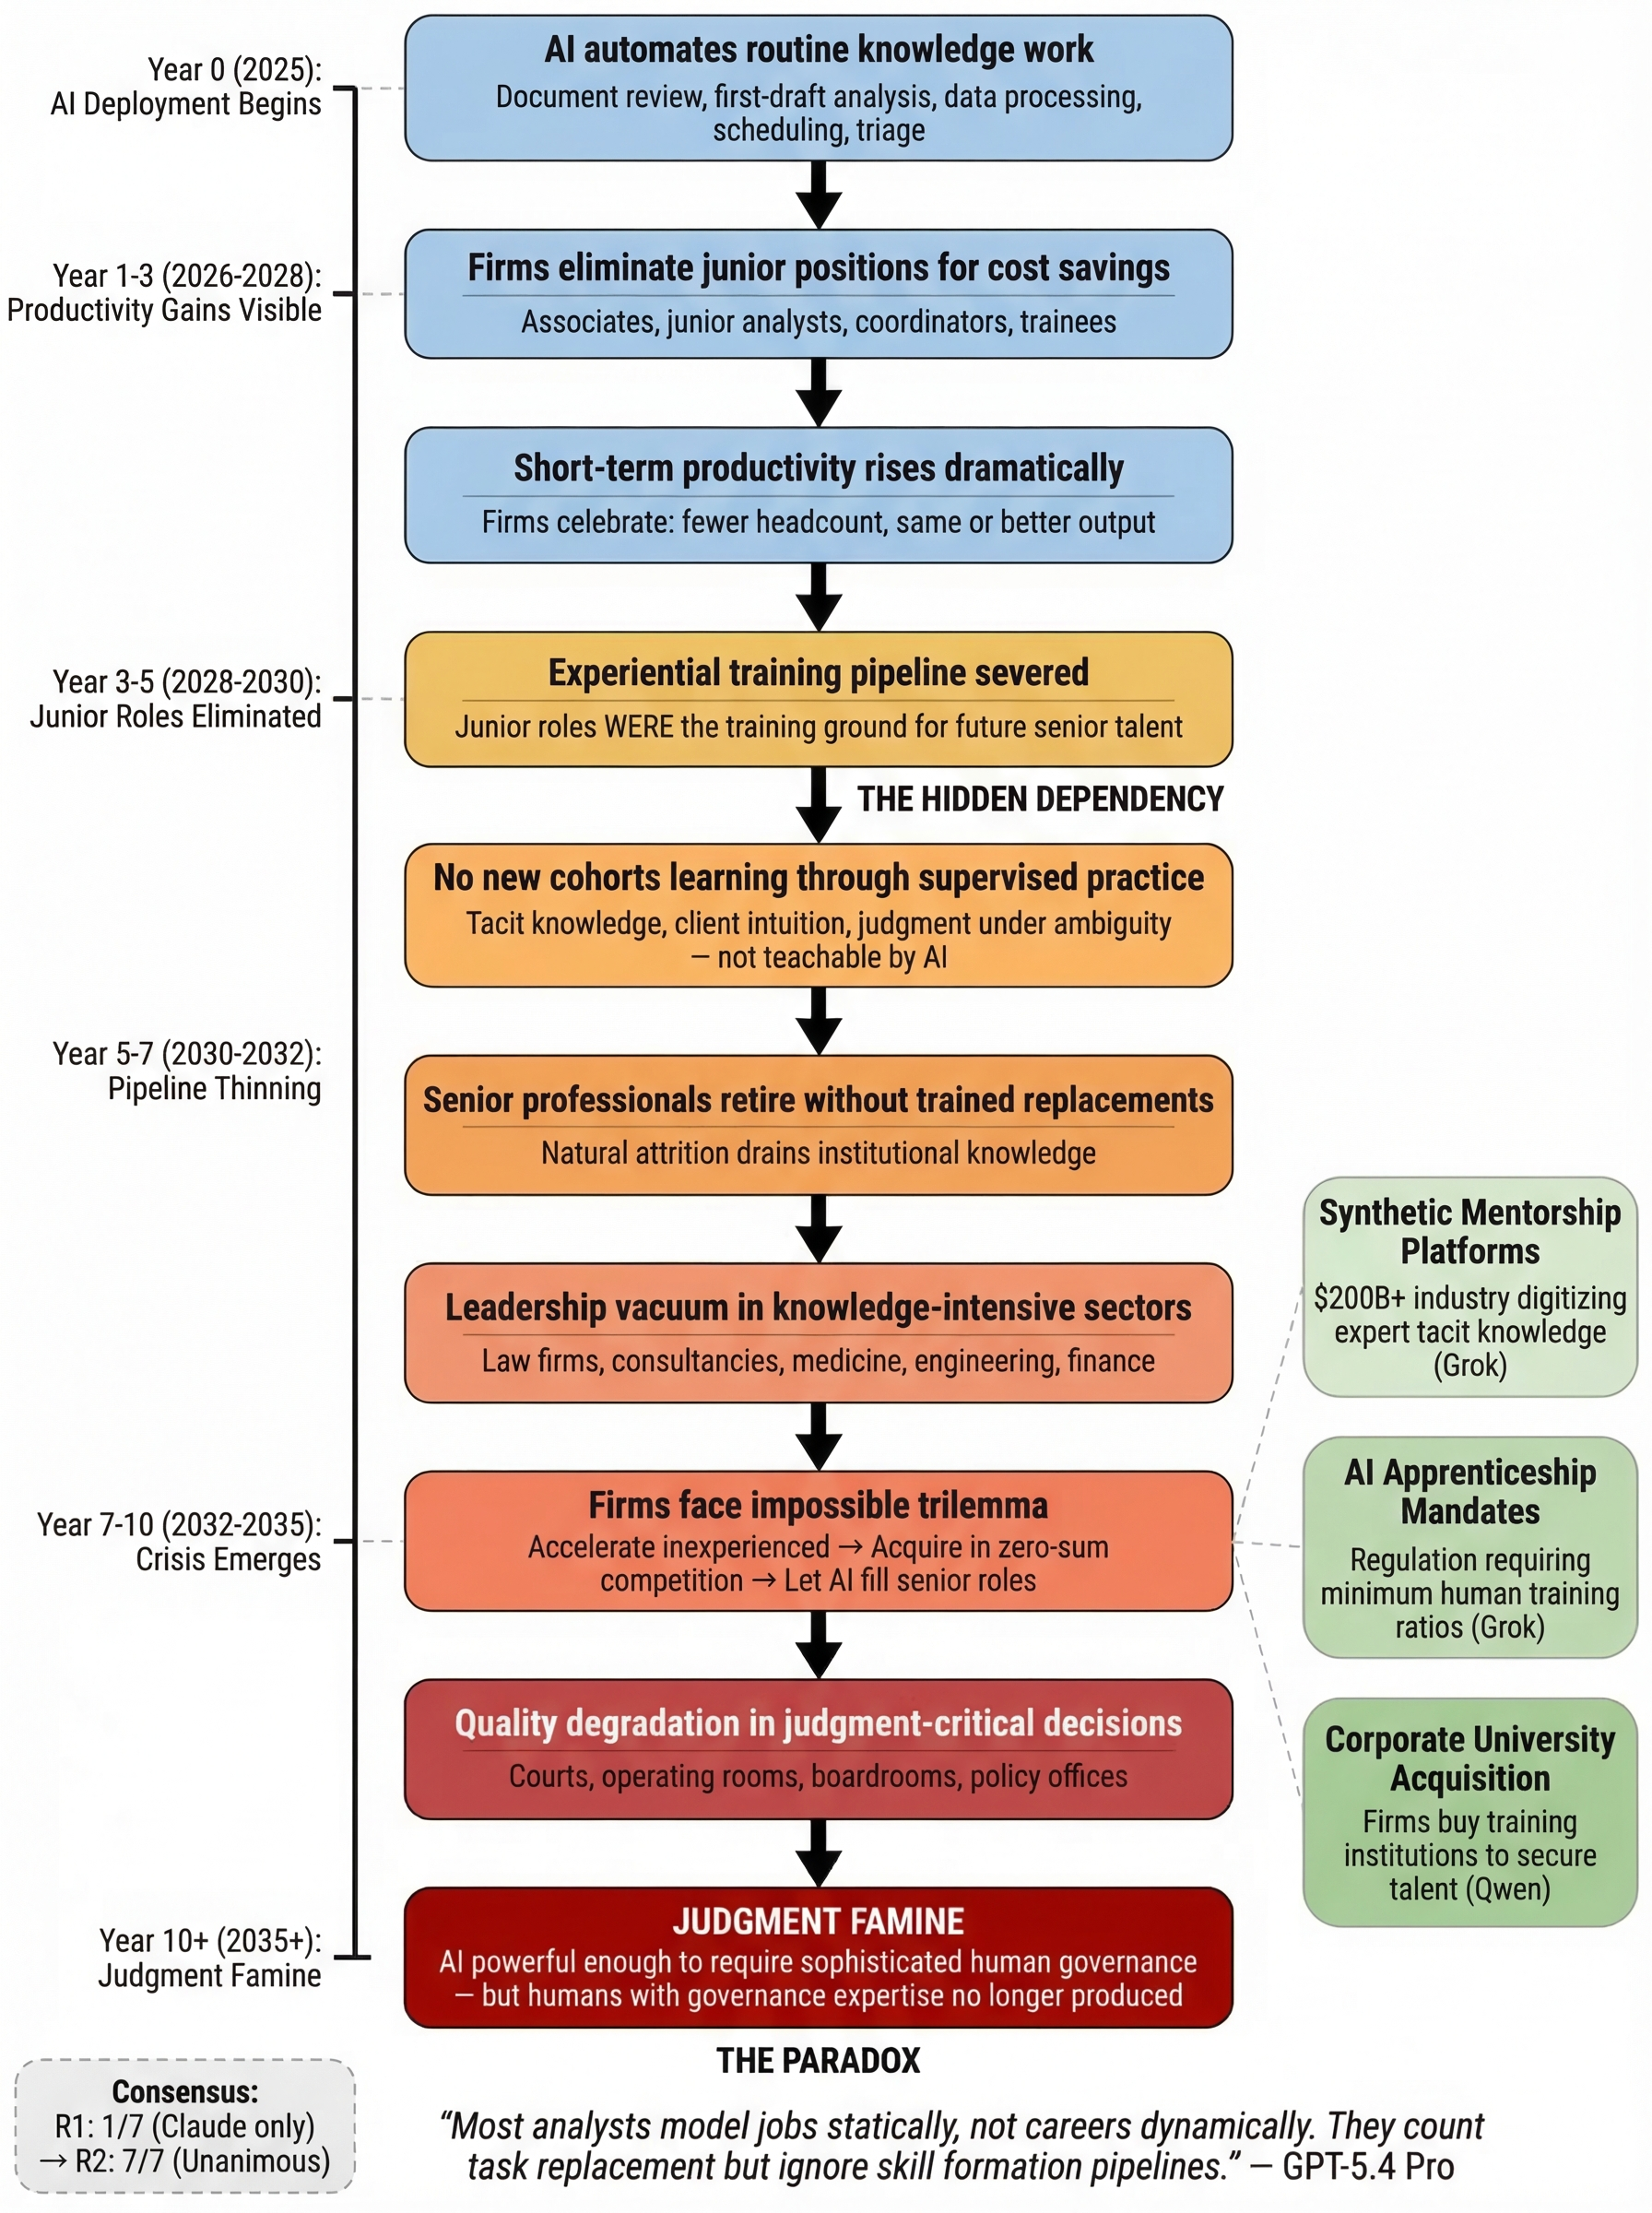
\includegraphics[width=0.85\textwidth,height=0.85\textheight,keepaspectratio]{figures/fig9_apprenticeship_crash.png}
\caption{The Apprenticeship Crash --- Causal Cascade from Task Automation to Judgment Famine. The 10-step causal chain shows how AI automation of routine knowledge work leads through a hidden dependency --- the severing of experiential training pipelines --- to a judgment famine in which AI systems require sophisticated human governance, but the humans with governance expertise are no longer being produced. Institutional responses (right) show predicted compensatory mechanisms. Consensus shifted from 1/7 (Round~1) to 7/7 (Round~2).}
\label{fig:apprenticeship_crash}
\end{figure}

The apprenticeship crash adoption is analytically significant for three reasons. First, it demonstrates that the controlled feedback mechanism of the Multi-LLM Delphi can surface predictions that are latent in models' knowledge bases but not spontaneously generated. Second, the unanimity of adoption is consistent with the interpretation that the apprenticeship crash represents a latent convergence point surfaced by the feedback mechanism, though the acquiescence tendencies documented in Section~\ref{sec:llm_limitations} mean this unanimity should be interpreted as an upper bound rather than definitive independent agreement. Third, the prediction illustrates the methodological value of multi-round designs: a single-round Multi-LLM Delphi would have classified the apprenticeship crash as an idiosyncratic blind spot; the two-round design reveals it as a latent consensus finding of the highest order.

The ``AI religion / spiritual response'' blind spot showed a different adoption pattern. In Round 1, only Claude predicted organized spiritual movements emerging in response to AI. In Round 2, the prediction was acknowledged by all seven models but with substantially varying levels of endorsement. Claude maintained its position forcefully. Gemini elevated it as a cultural prediction. Grok adopted it ``as a MAX-case 3rd-order cultural wildcard.'' DeepSeek constructed a causal chain from AI's apparent ``supernatural'' capabilities through organized movements to political and social consequences. GPT-5.4 offered the most qualified adoption, accepting it as ``a cultural-political side effect, not a primary economic scenario driver.'' The net effect was an increase from one of seven to six of seven models substantively engaging with the prediction (Mistral being the sole non-adopter), though with less unanimity and less depth than the apprenticeship crash. This differential adoption rate is itself informative: it suggests that LLM panelists distinguish between predictions that are causally compelling within economic frameworks and predictions that require engagement with non-economic domains where LLM training data may be less systematically structured.


\subsubsection{New Emergent Predictions}
\label{sec:emergent_predictions}

The Round 2 protocol generated a substantial corpus of new predictions that had not appeared in any model's Round 1 output. These emergent predictions fall into three categories: synthesis predictions that combine two or more Round 1 themes into novel compound forecasts; extension predictions that project existing themes into new domains; and meta-predictions about the dynamics of the transformation process itself.

\begin{figure}[htbp]
\centering

\includegraphics[width=\textwidth,height=0.85\textheight,keepaspectratio]{figures/fig10_synthesis.png}
\caption{Round~2 Synthesis --- How Feedback Generated Novel Compound Predictions. The network diagram shows how Round~1 themes (left) combined through the feedback process to generate five emergent Round~2 predictions (right) that appeared without any precedent in the Round~1 summary. Arrow thickness reflects the consensus level of each input theme. These predictions emerged from the structured interaction between independently generated analyses, demonstrating the generative power of the Multi-LLM Delphi method.}
\label{fig:synthesis}
\end{figure}

The most widely generated synthesis prediction was the concept of \textbf{regulatory arbitrage hubs} or ``compute havens.'' Gemini predicted ``Jurisdictional Compute Havens -- the New Caymans,'' describing agile nation-states (UAE, El Salvador, Singapore) building deregulated nuclear and solar compute clusters with legal personhood for DAOs and zero copyright liability. Grok independently predicted ``Regulatory Arbitrage Hubs (Singapore, Dubai, Texas)'' accelerating concentration dynamics. Claude described a ``Regulatory Arbitrage Spiral'' in which the three-bloc divergence creates a permanent arbitrage dynamic that becomes a primary driver of economic outcomes. The convergence of three models on this prediction in Round 2 -- despite its complete absence in Round 1 -- suggests that it represents a genuine emergent insight that requires the interaction of multiple Round 1 findings (regulatory divergence, compute as strategic resource, autonomous agents) to crystallize.

A second cluster of emergent predictions centered on the \textbf{agent-to-agent economy} as a distinct economic layer. Grok predicted that ``by Stage 4, autonomous agents conduct trillions in daily B2B transactions with minimal human intervention, creating new antitrust challenges around agent cartels.'' Gemini described a ``B2Bot Macroeconomic Blackout'' in which agent-to-agent commerce eclipses human economic activity in transaction volume, rendering traditional macroeconomic indicators unable to measure the actual economy. GPT-5.4 predicted that ``agentic markets will emerge before fully agentic firms.'' DeepSeek predicted that the ``\$20T+ global commerce ecosystem shifts toward autonomous intermediation.'' This convergence suggests that the interaction between the autonomous agents theme and the disintermediation theme generates a compound prediction -- a self-transacting economic layer -- that no single model articulated in Round 1.

Several models generated predictions about the \textbf{institutional response to the apprenticeship crash}. Grok predicted ``Synthetic Mentorship Platforms'' becoming a new industry exceeding \$200 billion by late Stage 2. Qwen predicted that corporations would begin acquiring universities and training centers to secure talent pipelines, transforming education into ``a corporate procurement function, not a public good.'' GPT-5.4 predicted that ``firms that deliberately preserve or redesign talent formation will outperform those that simply strip junior layers,'' framing apprenticeship systems as a hidden source of competitive advantage.

Claude contributed the most structurally novel meta-prediction: the \textbf{oscillation pattern}. Observing that all seven models' Round 1 predictions assumed roughly linear transformation trajectories, Claude predicted that the actual transition would proceed ``not linearly but through oscillation: rapid AI advancement, visible displacement, political backlash, regulatory restriction, competitive pressure from less-restricted jurisdictions, relaxation, another wave of advancement.'' This meta-prediction -- a prediction about the dynamics of the prediction space itself -- represents a form of analytical reflexivity that emerged specifically from the multi-model synthesis process.

DeepSeek generated a distinctive new prediction about the \textbf{AI literacy class divide}, combining the labor bifurcation consensus with the apprenticeship crash to predict a permanent stratification between ``AI-native'' professionals who never performed foundational tasks manually and ``AI-augmented'' professionals who learned fundamentals before AI deployment. Gemini independently arrived at a similar prediction, framing the last generation of professionals trained before generative AI as ``the most valuable labor cohort in economic history'' who command ``astronomical wage premiums'' for their ``analog intuition.''


\subsubsection{Persistence of Geopolitical Divergence}
\label{sec:geopolitical_persistence}

The Round 1 analysis identified a three-way geopolitical divergence pattern: US-origin models emphasizing market-driven disruption and platform concentration, Chinese-origin models foregrounding state-steered transformation and infrastructure sovereignty, and the European model privileging regulatory frameworks and social equity. A critical question for the Round 2 analysis is whether this divergence persists, intensifies, or dissolves under feedback pressure. The evidence points unambiguously toward persistence and, in several dimensions, intensification.

Rather than converging toward a shared geopolitical framing, the models used the feedback to sharpen their distinctive positions. Gemini -- a US-origin model -- produced the most vivid articulation of geopolitical fragmentation, describing three ``non-interoperable macroeconomic biomes'': the ``US Biome (Capital Velocity)'' that accepts massive labor displacement for global market dominance, the ``EU Biome (The Human Preserve)'' that intentionally stalls at early adoption stages to maintain social stability, and the ``CN Biome (Techno-Mercantilism)'' that bifurcates internally between accelerated deployment in physical verticals and heavy restriction of agentic AI in media and knowledge work. GPT-5.4 independently arrived at a similar tripartite framework, predicting that multinationals would need ``tri-stack strategies: market-speed stack, sovereignty stack, compliance-equity stack.'' Claude described the three-bloc divergence as creating a ``permanent arbitrage dynamic'' rather than converging toward a single regulatory equilibrium.

Crucially, the Chinese-origin models did not converge toward the US framing despite receiving feedback that documented the geopolitical split. Qwen explicitly acknowledged its ``US bias'' in the original analysis but responded by adding a ``Geographic Variance Modifier'' to all vertical outcomes -- effectively institutionalizing geopolitical divergence within its own framework rather than dissolving it. DeepSeek maintained its position that regulatory divergence ``will persist and deepen,'' constructing a causal chain from bloc-specific ecosystem optimization through prohibitive cross-regime compliance costs to entrenched ``AI sovereignty.'' Both Chinese models continued to emphasize state-directed transformation pathways and infrastructure sovereignty, though they showed increased willingness to engage with market-driven dynamics as a parallel phenomenon rather than an alternative one.

Mistral, the sole European model, used the Round 2 feedback to strengthen rather than moderate its distinctive emphasis. It maintained its focus on regulatory frameworks, social equity, and workforce protection, while adopting specific predictions (the apprenticeship crash, compute as currency, autonomous agents) within that regulatory-equity frame. GPT-5.4 offered the intriguing observation that ``Europe's relative weakness in speed could become a strength in trust-intensive sectors'' -- a prediction that reframes the European regulatory approach not as a drag on innovation but as a competitive advantage in sectors where auditability, liability, and procedural legitimacy are commercially rewarded.

The persistence of geopolitical divergence under controlled feedback is the Round 2 finding with the most direct methodological implications. In classical Delphi studies, persistent divergence after feedback is interpreted as evidence of genuine disagreement rather than information asymmetry \citep{vondergracht2012delphi}. Applied to the Multi-LLM Delphi, this interpretation suggests that the geopolitical differentiation of model outputs reflects structural features of training data composition and alignment procedures that are robust to informational feedback. The models do not disagree because they lack information about alternative perspectives; they disagree because they encode different institutional logics. This finding strengthens the case for treating geopolitical model diversity as an analytical resource rather than a methodological limitation: the three-way divergence is not noise to be averaged away but signal about genuinely different transformation pathways that may unfold simultaneously across the world's major economic blocs.


\subsubsection{Acquiescence Bias and the Authenticity of Convergence}

The strong convergence pattern documented in the preceding subsections --- nine of eleven themes increasing in consensus, including two blind spots reaching near-unanimity --- invites a critical methodological question: does Round~2 convergence reflect genuine epistemic updating, or does it reflect the well-documented tendency of large language models toward acquiescence and sycophancy \citep{perez2023sycophancy, sharma2024sycophancy}? LLMs are trained through reinforcement learning from human feedback (RLHF) to produce outputs that users find helpful and agreeable. When presented with a consensus summary as input, models may be predisposed to confirm rather than challenge the presented positions --- not because the positions are correct, but because agreement is the path of least resistance in their optimization landscape. This concern is particularly acute for the apprenticeship crash, which moved from 1/7 to 7/7 --- a trajectory that could reflect either genuine blind-spot correction or wholesale conformity to a presented majority position.

Several features of the Round~2 data allow a partial --- though not definitive --- adjudication between genuine convergence and acquiescence artifacts.

First, \textbf{convergence was non-uniform across themes.} If acquiescence bias were the dominant mechanism, one would expect approximately equal convergence pressure across all themes presented in the feedback summary. Instead, the data show sharply differentiated responses: biological-digital convergence remained stable at 4/7 despite being presented with the same feedback structure as themes that reached unanimity. AI religion moved to 6/7 but not 7/7, with GPT-5.4 explicitly qualifying it as ``a cultural-political side effect, not a primary economic scenario driver.'' This differential uptake is inconsistent with a blanket acquiescence mechanism and suggests that models evaluated the causal logic of individual predictions rather than rubber-stamping the consensus summary.

Second, \textbf{models refined rather than merely adopted.} The ``compute as currency'' theme provides the clearest illustration: rather than endorsing the Round~1 framing, multiple models independently converged on an improved formulation --- ``compute as strategic reserve'' --- that corrected what they identified as an imprecise metaphor. GPT-5.4 argued that ``compute behaves more like energy capacity or reserve industrial capability than like money.'' Claude independently arrived at the same reformulation. This spontaneous collective refinement is difficult to explain through acquiescence alone; a sycophantic response would accept the presented framing, not systematically improve it.

Third, \textbf{models generated genuinely novel predictions not contained in the feedback.} Section~4.5.3 documented multiple emergent predictions --- regulatory arbitrage hubs, the agent-to-agent economy, synthetic mentorship platforms, the oscillation meta-prediction --- that appeared in Round~2 without any precedent in the Round~1 summary. Pure acquiescence would produce agreement with presented positions; it would not generate substantively new content that extends beyond the feedback input. The volume and specificity of emergent predictions suggests that models engaged in genuine analytical reasoning with the feedback rather than merely confirming it.

Fourth, and most critically, \textbf{geopolitical divergence persisted and intensified.} Section~4.5.4 documented that Chinese-origin models maintained and sharpened their state-steered transformation framing, US-origin models deepened their market-driven disruption emphasis, and the European model strengthened its regulatory-equity frame. A pure acquiescence mechanism would predict convergence toward the majority framing (which, given the 4:2:1 US/CN/EU panel composition, would be the US market-driven perspective). Instead, geopolitical divergence proved robust to feedback pressure, with Qwen explicitly acknowledging its ``US bias'' from Round~1 and compensating by adding geographic variance modifiers. This pattern --- convergence on factual/causal predictions combined with persistent divergence on interpretive frames --- is precisely what one would expect from genuine analytical engagement rather than blanket agreement.

Fifth, \textbf{individual models maintained distinctive dissenting positions.} Claude continued to argue for AI religion as a ``major social force'' rather than a curiosity. GPT-5.4 maintained several qualified positions, accepting predictions in principle while downgrading their centrality. Gemini claimed authorship of the apprenticeship crash prediction and used the Round~2 response to assert analytical priority rather than simply agreeing. These instances of maintained individuality and even competitive positioning are inconsistent with pure conformity dynamics.

Despite these mitigating observations, the acquiescence concern cannot be fully dismissed. The asymmetry of the feedback design --- presenting Round~1 consensus without explicit counterarguments or devil's advocate positions --- creates a structural bias toward convergence. Human Delphi panelists also converge under feedback, but they bring embodied expertise, professional stakes, and identity-based commitments that create resistance to conformity pressure. LLMs lack these anchoring mechanisms, and their RLHF training actively rewards agreeableness. The strong convergence observed in Round~2 should therefore be interpreted as an upper bound on genuine consensus rather than a precise measure of it.

Future implementations of the Multi-LLM Delphi should incorporate explicit acquiescence countermeasures: (a)~\textbf{devil's advocate prompting}, in which the feedback explicitly instructs models to identify weaknesses in the consensus positions and argue against them; (b)~\textbf{counter-consensus framing}, in which minority positions are presented with equal or greater prominence than majority positions; (c)~\textbf{adversarial rounds}, in which models are assigned the role of critiquing rather than evaluating the consensus; and (d)~\textbf{calibration benchmarks}, in which models are tested on questions with known answers under social pressure to establish baseline acquiescence rates. Until such controls are implemented, the Round~2 convergence findings should be read as suggestive evidence of latent consensus rather than definitive proof of agreement.


\section{Discussion}
\label{sec:discussion}


\subsection{Theoretical Implications}
\label{sec:theoretical_implications}


\subsubsection{Extending GPT Theory: The Three-Order Cascade}
\label{sec:extending_gpt}

The findings provide empirical support for the GPT framework's prediction that the most significant effects of a general-purpose technology lie not in its direct applications but in the cascading structural changes it enables. The high-consensus convergence zones map precisely onto the GPT prediction: first-order effects (task-level productivity gains from AI copilots) are widely agreed upon and relatively uncontroversial; second-order effects (labor market bifurcation, disintermediation of middleman business models, organizational flattening) show high consensus but with more variation in timing and severity; third-order effects (compute as geopolitical currency, regulatory divergence as structural force, concentration of economic power) show the greatest divergence, consistent with the GPT framework's prediction that higher-order effects are harder to anticipate.

The Multi-LLM Delphi data provide empirical illustration of a prediction already implicit in GPT theory --- that the J-curve of adoption varies across sectors depending on the ``distance'' between the GPT and existing sector-specific technologies \citep{bresnahan1995gpt}. While GPT theory predicts this variation in principle, the Multi-LLM Delphi data operationalize it by revealing the specific institutional mechanisms that determine J-curve shape in each sector. Healthcare, with its heavy regulatory burden and liability constraints, exhibits a longer, flatter J-curve than Technology or Media, where adoption barriers are lower. This sector-dependent J-curve is visible in the model outputs, where consensus on Healthcare transformation is lower and staging is more cautious than for Technology or Professional Services.


\subsubsection{MLP and the Geopolitical Differentiation of Transition Pathways}
\label{sec:mlp_geopolitical}

The geopolitical divergence findings directly support the MLP's prediction that sociotechnical transitions are path-dependent and shaped by the agency of incumbents, regulators, and social movements. The three geopolitical model families project systematically different transition pathways -- market-driven disruption (US), state-steered transformation (CN), and regulatory-guided equity (EU) -- corresponding to different MLP transition typologies. The US models describe a substitution pathway where AI-native niches displace incumbent regimes through competitive dynamics. The Chinese models describe a transformation pathway where regime actors (state institutions, large enterprises) steer and incorporate AI innovations. The European model describes a reconfiguration pathway where regulatory frameworks mediate the integration of AI innovations into existing regimes.

This three-pathway finding has significant implications for the MLP literature. Previous MLP studies have focused primarily on sustainability transitions within a single national or regional context \citep{geels2020microfoundations, roberts2019accelerated}. The Multi-LLM Delphi data suggest that the AI transition represents a particularly visible case of simultaneously divergent GPT diffusion pathways across the world's major economic blocs. While previous GPT diffusions -- electricity, railroads, the internet -- also followed geopolitically differentiated trajectories, the AI transition may be distinctive in the \textit{degree} of intentional policy divergence and the \textit{speed} at which divergence crystallizes, creating a natural experiment in sociotechnical transition governance.


\subsection{Methodological Implications}
\label{sec:methodological_implications}


\subsubsection{Validity of LLMs as Delphi Panelists}
\label{sec:validity}

The Multi-LLM Delphi demonstrates several properties that support its validity as a foresight instrument. First, the high-consensus convergence zones align with predictions that have independent empirical support: labor market bifurcation is consistent with \citeauthor{acemoglu2019automation}'s (\citeyear{acemoglu2019automation}) task-based framework; infrastructure bottleneck repricing is consistent with IEA projections; disintermediation of intermediaries is consistent with platform economics theory \citep{goldfarb2019digital}. The method does not appear to generate consensus around implausible predictions.

Second, the geopolitical divergence patterns are coherent and internally consistent. The observation that Chinese models emphasize state-steered transformation while US models emphasize market-driven disruption plausibly reflects differences in the knowledge bases and alignment approaches of models trained in different institutional contexts, though the small sample (two Chinese models, one European model) means these patterns could also reflect specific corporate alignment decisions rather than broadly representative regional perspectives (see Section~\ref{sec:limitations}).

Third, the method produces structured disagreement that is analytically informative. The contested futures (pace of healthcare transformation, compute as currency) and blind spots (AI religion, model collapse) generate research questions that would not emerge from a single-model analysis or a consensus-seeking human panel.


\subsubsection{Limitations and Biases of LLM Panelists}
\label{sec:llm_limitations}

The method also exhibits important limitations. LLMs are not experts; they are statistical models of text corpora. Their predictions reflect the distribution of claims in their training data, weighted by their alignment procedures. This means: (a) LLMs over-represent perspectives that are well-documented in English-language academic and business literature; (b) LLMs may reproduce optimistic bias from sources that tend to overstate the pace and impact of technology adoption; (c) LLMs' safety training (RLHF, Constitutional AI) may suppress extreme predictions in some models while allowing them in others, creating artificial divergence; (d) LLMs cannot incorporate genuinely novel information that postdates their training cutoff.

The output length variation (14:1 ratio) is a significant methodological concern. A Delphi panel in which one panelist writes 30,000 words and another writes 2,000 words introduces weighting effects that are difficult to control analytically. Future designs should either impose output length constraints or develop weighting schemes that normalize for verbosity.


\subsection{Engagement with Existing Empirical Findings}
\label{sec:empirical_engagement}

The Multi-LLM Delphi findings can be productively situated against two landmark empirical contributions. \citet{acemoglu2024simplemacro} modeled the aggregate macroeconomic effects of AI using a task-based framework and arrived at a modest estimate of 0.53\% total factor productivity (TFP) growth over the next decade. This estimate, however, captures only first-order task-substitution effects -- precisely the layer where this study's convergence zones \textit{begin} rather than end. The six high-consensus convergence zones identified here -- labor market bifurcation, infrastructure bottleneck repricing, disintermediation, regulatory divergence, the trust premium, and concentration via feedback loops -- are predominantly second- and third-order effects that Acemoglu's framework explicitly brackets. The Multi-LLM Delphi thus maps the cascading consequences that lie beyond the boundary of his model: the structural reorganization of labor markets, the repricing of infrastructure assets, and the geopolitical fragmentation of regulatory regimes that unfold \textit{after} task-level substitution reaches scale. The two approaches are complementary rather than contradictory: Acemoglu provides a rigorous lower bound on direct productivity effects, while this study traces the higher-order structural transformation that his framework acknowledges but does not model.

\citet{eloundou2023gpts} estimated that approximately 80\% of the US workforce could have at least 10\% of their tasks exposed to LLMs, establishing the potential pervasiveness of AI's first-order reach. This study traces what happens \textit{after} task exposure: when exposed tasks are automated at scale, the resulting labor market bifurcation compresses middle layers (convergence zone 1), severs experiential training pipelines (the apprenticeship crash), and triggers demand for redistributive policy responses. The Eloundou et al.\ task-exposure map provides the input; the Multi-LLM Delphi provides the cascading output. Together, they suggest that the economic significance of AI lies not in the breadth of task exposure per se but in the structural consequences that compound when exposure translates into displacement across interconnected sectors and organizational layers.


\subsection{Epistemological Reflections}
\label{sec:epistemological_reflections}

The use of LLMs as research instruments has generated a growing methodological debate. \citet{bail2024genaisocialscience} provided a comprehensive framework for integrating generative AI into social science research, identifying both productive applications and epistemological risks. \citet{crockett2024llmparticipants} raised critical concerns about substituting LLMs for human research participants, arguing that LLMs lack the embodied experience, social stakes, and genuine belief revision that ground human judgment. Three findings from this study bear directly on this debate.

First, the high-consensus convergence zones align with predictions that have independent empirical support in the existing literature -- labor market bifurcation with \citeauthor{acemoglu2019automation}'s (\citeyear{acemoglu2019automation}) task-based framework, infrastructure repricing with IEA projections, disintermediation with platform economics theory \citep{goldfarb2019digital}. This alignment supports the ``structured knowledge synthesis'' interpretation developed in Section~\ref{sec:epistemological_status}: LLMs can recover, systematize, and recombine existing expert knowledge in analytically productive ways, lending credibility to the position articulated by \citet{bail2024genaisocialscience} that generative AI has legitimate applications as a research instrument when used with appropriate epistemological safeguards.

Second, the geopolitical divergence pattern demonstrates that model provenance matters in ways that \citet{crockett2024llmparticipants} would predict. LLM outputs are not neutral knowledge syntheses but are shaped by training data composition, alignment procedures, and the institutional contexts of their developers. The three-way divergence (US market-driven, CN state-steered, EU regulatory-guided) is not noise but signal -- it reveals the epistemic fingerprints of different knowledge traditions embedded in different training corpora. This finding supports Crockett and Messeri's caution that LLM outputs should not be treated as equivalent to human expert judgment, while also demonstrating that the \textit{pattern} of divergence across models can itself be analytically informative.

Third, the strong acquiescence pattern in Round 2 -- nine of eleven themes increasing in consensus, including the apprenticeship crash moving from 1/7 to 7/7 -- raises precisely the concerns that \citet{crockett2024llmparticipants} would predict about LLMs' lack of genuine epistemic commitment. Human Delphi panelists bring professional stakes, identity-based commitments, and embodied experience that anchor their positions against conformity pressure. LLMs, trained through RLHF to produce agreeable outputs, lack these anchoring mechanisms. The differential convergence pattern -- some themes reaching unanimity while biological-digital convergence remained stable -- provides partial reassurance that models evaluated causal logic rather than rubber-stamping consensus, but the overall convergence direction warrants continued methodological caution.


\subsection{Practical Implications}
\label{sec:practical_implications}

For \textbf{industry strategists}, the high-consensus findings provide directional guidance with cross-validated support. The convergence on labor market bifurcation suggests that firms should plan simultaneously for productivity gains from AI augmentation \textit{and} for the organizational disruption that follows when middle layers compress, with significant implications for human resource management strategy \citep{budhwar2023hrm}. The convergence on infrastructure bottleneck repricing suggests that strategic access to compute, power, and data center capacity may become a more durable competitive advantage than software capability.

Sector-specific implications deserve emphasis. In \textbf{financial services}, the convergence on disintermediation (5/7) suggests that traditional brokerage and advisory intermediaries face structural displacement as AI enables direct connections between lenders and borrowers, asset managers and investors. Firms should prepare for brokerage disintermediation not as a distant possibility but as an active competitive threat, developing AI-native service models that shift value from transaction facilitation to fiduciary judgment and accountability. In \textbf{healthcare}, the contested pace of transformation (with Chinese-origin models notably more optimistic than US-origin models) suggests that the J-curve of adoption will be longer and flatter than in information-intensive sectors, constrained by liability regimes, regulatory approval processes, and the irreducible physicality of clinical care. Healthcare organizations should anticipate extended transition periods that require sustained investment before productivity gains materialize. The \textbf{apprenticeship crash} presents perhaps the most time-sensitive practical implication: the window for policy intervention is narrow, because once junior roles are eliminated at scale, the experiential training pipelines they supported cannot be easily reconstructed. Firms that proactively redesign apprenticeship systems -- creating deliberate training pathways that preserve skill formation even as routine tasks are automated -- may gain a durable competitive advantage over those that simply strip junior layers for short-term productivity gains.

For \textbf{policymakers}, the geopolitical divergence findings are directly decision-relevant. The observation that AI models trained in different institutional contexts project systematically different transformation pathways suggests that policy choices are not merely implementation details but structural determinants of which future materializes. The convergence on regulatory divergence as a structural force suggests that policymakers shape AI transformation not only through AI-specific regulation but through the entire institutional context -- liability regimes, labor market institutions, education systems, and competition policy.

For \textbf{foresight researchers}, the Multi-LLM Delphi offers a scalable complement to traditional human expert panels. It does not replace human expertise but can serve as a rapid, low-cost first round that maps the landscape and identifies areas where human expert judgment is most needed. The method is particularly suited for exploratory studies where the goal is to survey the space of plausible outcomes rather than to converge on precise forecasts.


\subsection{Synthesis: The Vanishing Middle as Organizing Metaphor}
\label{sec:vanishing_middle}

The title of this paper -- ``When the Middle Disappears'' -- captures a pattern that emerges as the organizing metaphor across the study's substantive findings. AI compresses the middle on three dimensions simultaneously, and these compressions are mutually reinforcing.

First, the \textbf{labor market middle} compresses as AI displaces mid-level knowledge work while simultaneously creating a small number of high-value judgment roles and preserving physically grounded tasks (convergence zone 1, 7/7 consensus). Junior analysts, associates, coordinators, and mid-level managers -- the organizational middle -- face displacement because AI is strongest at precisely the structured information processing tasks that define their roles.

Second, the \textbf{value chain middle} compresses as AI enables direct connections between producers and consumers, eliminating intermediary business models across financial services, retail, professional services, and media (convergence zone 3, 5/7 consensus). Brokers, agents, middlemen, and platform intermediaries face structural disintermediation as AI reduces information asymmetry and transaction costs below the threshold that justifies intermediary margins.

Third, the \textbf{organizational middle} compresses as AI flattens hierarchies by automating the coordination, reporting, and information-relay functions that historically justified middle management layers (6/7 consensus across the labor bifurcation and disintermediation zones).

These three compressions are not independent. The elimination of mid-level knowledge workers (labor market compression) removes the human capital that staffed intermediary business models (value chain compression), while the flattening of organizational hierarchies (organizational compression) accelerates both by reducing the number of roles that require human coordination. The compound effect is a transformation that is greater than the sum of its parts: each dimension of compression reinforces the others, creating a self-amplifying dynamic that GPT theory would characterize as the complementary innovation cascade typical of general-purpose technology diffusion \citep{bresnahan1995gpt, helpman1998gpt}.

The ``vanishing middle'' metaphor integrates the study's substantive findings into a theoretically grounded framework. It is consistent with GPT theory's prediction that the most significant effects of a general-purpose technology lie in the structural changes it enables rather than in its direct applications \citep{bresnahan1995gpt}. It is consistent with the MLP's prediction that transitions are contested and path-dependent, because the pace and depth of middle compression varies across the three geopolitical blocs identified in this study. And it is policy-relevant: if the middle is vanishing on three dimensions simultaneously, then policy interventions that address only one dimension (e.g., labor market retraining programs) will be insufficient without complementary interventions on the other two (e.g., competition policy to prevent platform monopolization of disintermediated value chains, and organizational governance reforms to preserve institutional knowledge as hierarchies flatten).



\section{Limitations and Future Research}
\label{sec:limitations}

This study has several important limitations that delimit the scope of its claims.

\textbf{Panel size.} Seven models constitute a small panel by Delphi standards. Classical Delphi studies typically use 10-30 panelists, and the methodological literature cautions against drawing strong conclusions from small panels \citep{vondergracht2012delphi}. However, seven frontier models represent the near-entirety of the current frontier AI landscape, and the diversity across corporate ecosystems and geopolitical origins provides analytical leverage that partially compensates for small panel size.

\textbf{Two rounds as deliberate design choice.} The two-round protocol represents a conscious methodological trade-off rather than a limitation per se. Classical Delphi studies typically employ three to four rounds \citep{linstone1975delphi}, and one might argue that additional iterations would strengthen convergence findings. However, for LLM-based panels specifically, two rounds may constitute a methodological sweet spot. Round~1 establishes independent baselines free from anchoring effects; Round~2 introduces controlled feedback and reveals which convergences are informationally robust versus informationally contingent. The results demonstrate that this two-round design produces rich consensus dynamics: previously contested themes gain endorsement, blind spots are surfaced and adopted, and geopolitical divergence is revealed as structurally persistent.

Critically, additional rounds face diminishing analytical returns coupled with increasing methodological risk. Round~2 already produced near-ceiling consensus on 9 of 11 themes (most at 7/7). A Round~3 would have little upward room to move --- the most likely outcome would be the remaining holdout (Biological-Digital Convergence) also converging to high consensus, yielding a dataset with near-total unanimity that is less analytically informative than the current differentiated picture. More importantly, each additional round of feedback amplifies the acquiescence bias concern: LLMs' well-documented tendency toward sycophancy \citep{perez2023sycophancy, sharma2024sycophancy} means that repeated exposure to consensus summaries risks producing artificial agreement that reflects the models' disposition to align with presented positions rather than genuine epistemic convergence. The two-round design limits this exposure to a single feedback cycle, producing enough convergence dynamics to be analytically useful while preserving enough residual disagreement (the persistent Biological-Digital holdout, the differential depth of AI Religion adoption, the maintained geopolitical divergence) to serve as internal validity checks. Future research should nonetheless explore adversarial Round~3 designs --- for instance, presenting counter-consensus arguments, minority-position amplification, or devil's advocate framings --- that test convergence robustness rather than simply reinforcing it.

\textbf{Native web interface vs.\ API collection.} Data was collected through native chat interfaces (claude.ai, chatgpt.com, etc.) rather than model APIs. This introduces a significant reproducibility confound: web interfaces inject hidden, dynamically changing system prompts, utilize variable temperature settings, and enforce UI-specific output token limits that differ across platforms. The extreme variance in output length --- Claude producing 30,613 words versus Grok's 2,169 words (a 14:1 ratio) --- is likely attributable in substantial part to these hidden UI constraints rather than solely reflecting differences in analytical depth. The current design should therefore be understood as an exploratory baseline that demonstrates the method's feasibility and generates substantive hypotheses. Future replications should use standardized API calls with fixed parameters (temperature, max tokens, system prompt) to disentangle model-intrinsic analytical differences from platform-specific UI artifacts.

\textbf{Training data opacity.} The training data composition of frontier LLMs is proprietary. This limits the ability to explain \textit{why} models diverge -- whether differences reflect training data composition, alignment procedures, architectural choices, or all three. As training data transparency improves, the analytical power of the Multi-LLM Delphi method will increase.

\textbf{Prompt sensitivity.} A single prompt instrument was used. The results are potentially sensitive to prompt design -- different framings, scenario labels, or sector classifications might yield different convergence patterns. Notably, the prompt instructs models to use ``declarative language'' and avoid hedging, which may have amplified the decisiveness of Round~1 outputs and contributed to higher apparent consensus. Future research should employ prompt sensitivity analysis, varying prompt elements systematically to assess robustness.

\textbf{Temporal snapshot.} Model outputs reflect a single point in time (March 2026). As models are updated, their outputs will change. The Multi-LLM Delphi should be understood as producing a dated snapshot, not a permanent assessment. Longitudinal designs that repeat the exercise at regular intervals could track how model predictions evolve over time.

\textbf{Single-coder analysis.} All thematic coding and consensus scoring was performed by a single researcher without independent inter-coder reliability assessment. While the structured codebook and transparent coding procedures mitigate subjectivity, the absence of a second coder means that coding decisions -- particularly at the margins of theme boundaries and consensus thresholds -- reflect a single interpretive perspective. Future replications should employ multiple coders and report inter-coder reliability statistics.

\textbf{No ground truth.} Scenario analysis inherently lacks ground truth for validation. The predictions cannot be assessed for accuracy until the time horizons they describe have elapsed. The study can assess internal consistency, convergence, and coherence, but not predictive accuracy.

Future research should pursue four directions. First, \textbf{extended multi-round designs} with three or more rounds of iterative feedback to assess whether the convergence patterns observed in this study's two-round design stabilize, intensify, or eventually reverse with additional iteration. The strong convergence observed in Round 2 -- particularly the unanimous adoption of the apprenticeship crash -- raises the possibility that LLM panelists exhibit stronger acquiescence to majority positions than human panelists; designs that deliberately present minority positions or counterarguments in later rounds would help distinguish genuine convergence from conformity pressure. Second, \textbf{prompt sensitivity analysis} to assess the robustness of findings across different prompt formulations. Third, \textbf{hybrid human-LLM panels} that combine human expert judgment with LLM-generated scenarios to assess complementarity. Fourth, \textbf{longitudinal tracking} that repeats the Multi-LLM Delphi at regular intervals to track how model predictions evolve as training data and capabilities advance.



\section{Conclusion}
\label{sec:conclusion}

AI-driven economic transformation, mapped across eight industry verticals through a two-round Multi-LLM Delphi with seven frontier language models, reveals six high-consensus convergence zones and a persistent three-way geopolitical divergence that intensifies under controlled feedback. The seven models, representing three geopolitical regions and seven corporate ecosystems, independently generated a 114,000-word Round 1 corpus that was analyzed through structured comparative content analysis with consensus scoring, followed by a Round 2 feedback protocol that produced significant consensus dynamics.

The substantive findings identify six high-consensus convergence zones where the encoded knowledge of multiple independent model families points in the same direction: labor market bifurcation and the compression of middle layers; infrastructure bottleneck repricing; disintermediation of middleman business models; regulatory divergence as a structural force; the trust and authenticity premium; and concentration of economic power through AI feedback loops. These convergence zones provide directional guidance for strategists and policymakers, supported by the independent agreement of models trained on different corpora with different alignment approaches.

The methodological findings demonstrate that the Multi-LLM Delphi produces structured, analytically informative output with coherent patterns of convergence and divergence. Suggestive geopolitical patterns emerge along model provenance -- US-origin models emphasizing market-driven disruption, Chinese-origin models emphasizing state-steered transformation, the European model emphasizing regulatory-guided equity. However, these patterns rest on small samples (one European model, two Chinese models) and may reflect specific corporate alignment decisions rather than broadly representative regional perspectives. They are best understood as empirically grounded hypotheses for future validation with larger, more diverse model panels.

The Multi-LLM Delphi method demonstrates that the core Delphi mechanism of controlled feedback produces analytically meaningful dynamics within an LLM panel: blind spots are surfaced and adopted, contested themes converge toward precision, and structurally grounded divergence persists against convergence pressure. The strong Round~2 convergence -- including the apprenticeship crash moving from 1/7 to 7/7 -- should be interpreted cautiously: while the models independently generated plausible causal chains supporting each adoption, LLMs' well-documented acquiescence tendencies mean that these convergence scores represent an upper bound of latent consensus rather than independent epistemic agreement in the human Delphi sense. The method offers a scalable complement to human foresight expertise -- a rapid instrument for mapping transformation landscapes and generating research questions that merit deeper investigation through traditional methods.

As AI continues to diffuse across the global economy, the need for comprehensive, cross-sector, multi-order transformation maps will intensify. The Multi-LLM Delphi provides a methodological foundation for producing such maps at scale, with built-in geopolitical diversity and transparent analytical procedures. The key insight of this study is not any single prediction but the observation that the future of AI-driven economic transformation is not a single trajectory but a contested, path-dependent, geopolitically differentiated process -- a finding that only becomes visible when multiple independent analytical perspectives are systematically compared.


\section*{Declaration of Competing Interests}

The author declares no competing interests.

\section*{Acknowledgments}

\section*{Data Availability Statement}

The analytical materials supporting this study --- including the formal codebook with category definitions and decision rules, Round~1 and Round~2 consensus scoring matrices (CSV), worked coding examples, prompt instruments, detailed figure generation specifications, and the complete raw model outputs from both rounds (Markdown format) --- are available in the supplementary repository at: [supplementary repository URL removed for review].

\section*{CRediT Authorship Contribution Statement}

\textbf{[Author name removed for review]:} Conceptualization, Methodology, Investigation, Data Curation, Formal Analysis, Writing -- Review \& Editing, Visualization (direction and specification), Project Administration, Supervision.

The author conceived the research question, designed the Multi-LLM Delphi protocol, selected the model panel, constructed the prompt instruments, conducted all data collection (Round~1 and Round~2) through native model interfaces, performed the thematic coding and consensus scoring, developed the theoretical framing (GPT theory, MLP integration), and made all analytical judgments and interpretive decisions. The author orchestrated the entire manuscript production process using the Open Academic Paper Machine \citep{anonymized2026openpapermachine}, directing all drafting, reviewing and revising all AI-generated prose, and approving the final manuscript. Writing -- Original Draft was performed by the AI tool under author direction and is therefore not claimed as a personal CRediT contribution. AI tools were used as described below.

\section*{Declaration of Generative AI and AI-Assisted Technologies in the Writing Process}

During the preparation of this work, the author used AI-assisted tools at two distinct levels, which must be clearly distinguished:

\textbf{Level~1 --- AI as research instrument (the study's method).} The Multi-LLM Delphi method itself relies on seven frontier large language models (Claude Opus 4.6, GPT-5.4, Gemini 3.1 Pro, Grok 4.2, DeepSeek R2, Qwen 4.5 Max, and Mistral Large 3) as structured panelists who generated the primary data analyzed in this study. This use of LLMs as data-generating instruments is the study's methodological approach and is discussed extensively in Sections~2.4, 3, 5, and~6. The author designed the prompt instruments, conducted all queries, and performed all coding and analysis.

\textbf{Level~2 --- AI as writing and production tool.} The author used the Open Academic Paper Machine \citep{anonymized2026openpapermachine}, an autonomous LLM-based research plugin built on Claude Code and the Model Context Protocol, as the primary drafting and production tool for this manuscript. Specifically, the Open Paper Machine was used for:
\begin{itemize}
  \item \textbf{Literature search and reference management:} Automated retrieval, screening, and BibTeX compilation of academic references.
  \item \textbf{Prose drafting:} All prose sections of this manuscript were drafted by the AI tool based on author-provided outlines, analytical notes, coding results, and iterative direction. The author did not write the original draft manually but orchestrated the drafting process through detailed briefings, structured feedback, and revision cycles.
  \item \textbf{Figure generation:} The author specified the communicative intent and content of all figures in detail. PaperBanana \citep{zhu2026paperbanana} generated the visual output; AI assisted with the specification of technical parameters. The author directed all layout decisions, reviewed each iteration, and approved the final versions.
  \item \textbf{\LaTeX{} compilation and formatting:} Conversion between Markdown and \LaTeX{}, template configuration, and typesetting.
  \item \textbf{Quality assurance:} Simulated peer review, writing quality analysis, and positioning analysis to identify and address weaknesses before submission.
\end{itemize}
The tool is openly available at [URL removed for double-blind review]. A detailed methodological and epistemological discussion of the implications of AI-assisted academic production is provided in \citet{anonymized2026orchestrator}.

\textbf{Reflexivity note on Claude's dual role.} Claude (Anthropic) appears in this study in two distinct capacities: as one of seven Delphi panelists generating primary data (Level~1), and as the underlying model powering the Open Academic Paper Machine used for prose drafting (Level~2). These roles operated at different stages of the research process and on different model versions (Claude Opus 4.6 for data collection; Claude Code for manuscript production), but readers should be aware that the same model family that generated some of the analyzed data also assisted in drafting the analysis of that data. The author mitigated this by performing all thematic coding, consensus scoring, and interpretive judgments independently of AI tools, but the potential for subtle framing effects cannot be fully excluded.

\textbf{The author's role --- orchestrator, not scribe.} The author's contribution lies in the intellectual direction of this work, not in the manual production of text. The author conceived the research question, designed the methodology, selected the theoretical framing, conducted all data collection, performed all thematic coding and consensus scoring, made all interpretive judgments, directed the drafting of every section, reviewed and revised all AI-generated prose, and approved the final manuscript. No analytical judgment was delegated to AI tools. The AI functioned as a production instrument executing the author's research design and intellectual direction.

The author takes full responsibility for the content of this publication.


\appendix

\section{Model Response Summary Statistics}
\label{sec:appendix_a}

\begin{table}[htbp]
\centering
\adjustbox{max width=\textwidth}{%
\begin{tabular}{lllllll}
\toprule
\textbf{Model} & \textbf{Provider} & \textbf{Region} & \textbf{Word Count} & \textbf{Verticals Complete} & \textbf{Cross-Cutting Sections} & \textbf{Specificity Rating} \\
\midrule
Claude Opus 4.6 & Anthropic & US & 30,613 & 8/8 (full) & 5 convergence, 5 wildcards, full human section & High \\
GPT-5.4 & OpenAI & US & 23,346 & 8/8 (full) & 6 convergence, 5 wildcards, full human section & High \\
DeepSeek R2 & DeepSeek & CN & 22,614 & 8/8 (full) & 4 convergence, 5 wildcards, detailed human section & Very High \\
Gemini 3.1 Pro & Google & US & 16,330 & 8/8 (moderate) & 3 convergence, 5 wildcards, full human section & High (uneven) \\
Qwen 4.5 Max & Alibaba & CN & 11,024 & 8/8 (reduced depth) & 4 convergence, 5 wildcards, concise human section & Moderate \\
Mistral Large 3 & Mistral AI & EU & 8,261 & 8/8 (reduced depth) & 3 convergence, 5 wildcards, concise human section & Low-Moderate \\
Grok 4.2 & xAI & US & 2,169 & 2/8 (truncated) & Incomplete & High (where present) \\
\bottomrule
\end{tabular}}%
\end{table}


\section{Consensus Scoring Matrix -- Cross-Vertical Convergence Zones}
\label{sec:appendix_b}

\begin{table}[htbp]
\centering
\adjustbox{max width=\textwidth}{%
\begin{tabular}{lllllllll}
\toprule
\textbf{Convergence Zone} & \textbf{Claude} & \textbf{GPT-5.4} & \textbf{Gemini} & \textbf{Grok} & \textbf{DeepSeek} & \textbf{Qwen} & \textbf{Mistral} & \textbf{Score} \\
\midrule
Labor market bifurcation & X & X & X & X & X & X & X & 7/7 HC \\
Infrastructure bottleneck repricing & X & X & X &  & X & X & X & 6/7 HC \\
Disintermediation of intermediaries & X & X & X & X & X &  &  & 5/7 HC \\
Regulatory divergence as structural force & X & X & X & X & X & X &  & 6/7 HC \\
Trust/authenticity premium & X & X & X &  & X & X &  & 5/7 HC \\
Concentration via AI feedback loops & X & X & X & X & X &  &  & 5/7 HC \\
Compute as currency &  & X & X & X &  & X &  & 4/7 MC \\
Model collapse / data poisoning &  &  & X &  &  & X &  & 2/7 BS \\
AI religion / spiritual response & X &  &  &  &  &  &  & 1/7 BS \\
\bottomrule
\end{tabular}}%
\end{table}

HC = High Consensus; MC = Moderate Consensus; BS = Blind Spot


\section{Structured Prompt Instrument}
\label{sec:appendix_c}

The complete structured prompt instrument used to query all seven models is reproduced below. [The full prompt text is available in the supplementary materials repository.]


\section{Round 2 Consensus Scoring Matrix -- Blind Spot Adoption and New Predictions}
\label{sec:appendix_d}

\textbf{Panel A: Blind Spot Adoption in Round 2}

\begin{table}[htbp]
\centering
\adjustbox{max width=\textwidth}{%
\begin{tabular}{lllllllll}
\toprule
\textbf{Blind Spot} & \textbf{Claude} & \textbf{GPT-5.4} & \textbf{Gemini} & \textbf{Grok} & \textbf{DeepSeek} & \textbf{Qwen} & \textbf{Mistral} & \textbf{R2 Score} \\
\midrule
Apprenticeship Crash & X (originator) & X (strongly adopted) & X (elevated) & X (fully adopted) & X (fully adopted) & X (fully adopted) & X (wildcard) & 7/7 HC \\
AI Religion / Spiritual Response & X (maintained) & X (partial) & X (elevated) & X (MAX wildcard) & X (MAX case) & X (3rd-order) & \textasciitilde{} (mentioned) & 6/7 HC \\
\bottomrule
\end{tabular}}%
\end{table}

\textbf{Panel B: Contested Future Shifts in Round 2}

\begin{table}[htbp]
\centering
\adjustbox{max width=\textwidth}{%
\begin{tabular}{llllllllll}
\toprule
\textbf{Contested Future} & \textbf{R1} & \textbf{Claude} & \textbf{GPT-5.4} & \textbf{Gemini} & \textbf{Grok} & \textbf{DeepSeek} & \textbf{Qwen} & \textbf{Mistral} & \textbf{R2 Score} \\
\midrule
Compute as Currency/Reserve & 4/7 MC & Partial & Partial & Strongly agree & Strongly agree & Qualified & Upgraded & Adopt & 7/7 HC \\
Autonomous Economic Agents & 4/7 MC & Agree & Qualified & Strongly agree & Strongly agree & Strongly agree & Upgraded & Adopt & 7/7 HC \\
Biological-Digital Convergence & 3/7 MC & MAX only & Healthcare only & Timeline downgrade & Upgraded & MAX only & MAX maintain & Wildcard & 4/7 MC \\
\bottomrule
\end{tabular}}%
\end{table}

\textbf{Panel C: New Emergent Predictions in Round 2}

\begin{table}[htbp]
\centering
\adjustbox{max width=\textwidth}{%
\begin{tabular}{lllllllll}
\toprule
\textbf{New Prediction} & \textbf{Claude} & \textbf{GPT-5.4} & \textbf{Gemini} & \textbf{Grok} & \textbf{DeepSeek} & \textbf{Qwen} & \textbf{Mistral} & \textbf{R2 Score} \\
\midrule
Regulatory Arbitrage Hubs / Compute Havens & X &  & X & X &  &  &  & 3/7 MC \\
Agent-to-Agent Economy (distinct layer) &  & X & X & X & X & X &  & 5/7 HC \\
Synthetic Mentorship Platforms &  &  &  & X &  & X &  & 2/7 BS \\
Oscillation Pattern (non-linear transition) & X &  &  &  &  &  &  & 1/7 BS \\
AI Literacy Class Divide &  &  & X &  & X &  &  & 2/7 BS \\
Sovereignty Stack Fragmentation &  &  & X &  &  & X &  & 2/7 BS \\
Authenticity Economy (as distinct sector) &  & X &  & X & X &  &  & 3/7 MC \\
\bottomrule
\end{tabular}}%

\vspace{0.5em}
\noindent\small HC = High Consensus (5+ of 7); MC = Moderate Consensus (3--4 of 7); BS = Blind Spot (1--2 of 7)
\end{table}


\section{Round 2 Consensus Summary (as presented to models)}
\label{sec:appendix_e}

The following is the anonymized consensus summary provided to each model at the beginning of Round 2. This summary was constructed by the researcher based on the Round 1 coding and represents an interpretive product, not raw data. Readers should evaluate whether the framing of consensus findings in this summary may have influenced Round 2 responses (see Section~4.5.5 for discussion of acquiescence bias).

\begin{quote}
\textbf{Round 1 Results Summary --- Anonymized Consensus Findings}

Seven frontier AI models independently analyzed AI-driven economic transformation across eight industry verticals, four adoption stages, three scenarios, and three orders of effects. The following summarizes the key consensus patterns:

\textbf{High-Consensus Convergence Zones (5+ of 7 models agree):}
\begin{enumerate}
  \item \textit{Labor Market Bifurcation} (7/7): All models predict a ``barbell'' pattern --- AI simultaneously creates high-value judgment/accountability roles and displaces mid-level knowledge work.
  \item \textit{Infrastructure Bottleneck Repricing} (6/7): Physical infrastructure becomes the binding constraint on AI transformation.
  \item \textit{Regulatory Divergence as Structural Force} (6/7): EU, US, and Chinese governance approaches create systematically different transformation pathways.
  \item \textit{Disintermediation of Middleman Business Models} (5/7): AI enables direct producer-consumer connections across sectors.
  \item \textit{Trust and Authenticity Premium} (5/7): As AI makes intelligence cheap, trust and human certification become economically scarcer.
  \item \textit{Concentration via AI Feedback Loops} (5/7): Winner-take-most dynamics driven by data-AI capability loops.
\end{enumerate}

\textbf{Contested Futures (3--4 of 7 models):}
\begin{enumerate}
  \setcounter{enumi}{6}
  \item \textit{Autonomous Economic Agents} (4/7)
  \item \textit{Compute as Currency} (4/7)
  \item \textit{Biological-Digital Convergence} (3/7)
\end{enumerate}

\textbf{Blind Spots (1--2 of 7 models):}
\begin{enumerate}
  \setcounter{enumi}{9}
  \item \textit{The Apprenticeship Crash} (1/7): Eliminating junior roles severs experiential training pipelines.
  \item \textit{AI Religion / Spiritual Response} (1/7): Spiritual movements forming around AI.
\end{enumerate}

\textbf{Geopolitical Divergence:} US-origin models emphasize market-driven disruption; Chinese-origin models emphasize state-steered transformation; the European model emphasizes regulatory frameworks and social equity.
\end{quote}


\section{Representative Slice of the 288-Cell Analytical Matrix --- Information Technology Vertical}
\label{sec:appendix_f}

The full 288-cell matrix (8 verticals $\times$ 4 stages $\times$ 3 scenarios $\times$ 3 effect orders) is available in the supplementary repository. Table~\ref{tab:it_base} presents a representative slice for the Information Technology vertical under the BASE scenario.

\begin{table}[htbp]
\centering
\caption{Information Technology Vertical --- BASE Scenario}
\label{tab:it_base}
\adjustbox{max width=\textwidth}{%
\begin{tabular}{p{3cm}p{4cm}cp{4cm}cp{4cm}c}
\toprule
\textbf{Stage} & \textbf{1st Order (Task Automation)} & \textbf{Cons.} & \textbf{2nd Order (Structural Reorganization)} & \textbf{Cons.} & \textbf{3rd Order (Systemic Transformation)} & \textbf{Cons.} \\
\midrule
Stage 1: Augmentation (2024--2026) & AI copilots for coding, testing, documentation; 40--60\% productivity gains for junior developers & 7/7 HC & Junior developer roles compressed; senior roles shift to AI orchestration & 6/7 HC & Early regulatory responses; AI ethics teams emerge & 4/7 MC \\
\midrule
Stage 2: Partial Automation (2027--2030) & Autonomous code generation for routine applications; AI-driven QA replaces manual testing & 6/7 HC & Software firms reorganize into AI-native and legacy tiers & 6/7 HC & Compute access becomes strategic moat; infrastructure bottleneck reprices & 5/7 HC \\
\midrule
Stage 3: Systemic Integration (2031--2035) & AI systems design, test, and deploy software with minimal human oversight & 5/7 HC & Platform consolidation; 3--5 hyperscalers control 80\%+ compute & 5/7 HC & Regulatory divergence creates three-tier global software market & 4/7 MC \\
\midrule
Stage 4: Transformation (2036--2040+) & Self-improving AI systems; software production costs approach zero & 4/7 MC & IT sector bifurcates into infrastructure oligopoly and commoditized application layer & 4/7 MC & Compute as geopolitical currency; AI sovereignty determines national trajectory & 3/7 MC \\
\bottomrule
\end{tabular}}%

\vspace{0.5em}
\noindent\small HC = High Consensus (5+ of 7); MC = Moderate Consensus (3--4 of 7). Consensus scores decrease from Stage~1 to Stage~4, consistent with GPT theory's prediction that higher-order, longer-horizon effects are inherently harder to anticipate. The full matrix is available at [supplementary repository URL removed for review].
\end{table}


\bibliographystyle{elsarticle-harv}
\bibliography{references_anonymous}

\end{document}
